\documentclass[12pt]{article}
\usepackage{graphicx}
\usepackage{float}
\usepackage{subcaption}
\usepackage{hyperref}
\usepackage{mathtools}
\usepackage[usenames,dvipsnames]{xcolor}
\usepackage[authoryear]{natbib}
\usepackage{amsmath}
\usepackage{amsfonts}
\usepackage{bigints}
\usepackage{array}
\usepackage{tikz}
\usepackage{longtable}
\usepackage{geometry}

\bibliographystyle{plainnat}

\setlength{\parskip}{\baselineskip}
\setlength{\parindent}{0pt}

\newcommand{\e}[1]{{\mathbb E}\left[ #1 \right]}
\newcommand{\given}{\mid}
\newcommand{\secref}[1]{``\nameref{#1}''}
\newcommand{\tri}{\textit{trichocarpa}} 
\newcommand{\bals}{\textit{balsamifera}}


\newcommand{\R}{\mathbb{R}}
\newcommand{\Q}{\mathbb{Q}}
\newcommand{\Z}{\mathbb{Z}}
\newcommand{\N}{\mathbb{N}}
\newcommand{\C}{\mathbb{C}}

\renewcommand{\P}{\mathbb{P}}
\newcommand{\E}{\mathbb{E}}
\newcommand{\var}{\mathop{\mbox{Var}}}
\newcommand{\cov}{\mathop{\mbox{cov}}}
%\newcommand{\det}{\mathop{\mbox{det}}}
\newcommand{\supp}{\mathop{\mbox{supp}}}
\newcommand{\sgn}{\mathop{\mbox{sgn}}}
\newcommand{\EE}[1]{\E\!\left[#1\right]}
\newcommand{\PP}[1]{\P\!\left\{#1\right\}}
\newcommand{\PPP}[2]{\P_{#1}\!\left\{#2\right\}}
\newcommand{\EEE}[2]{\E_{#1}\!\left[#2\right]}
\newcommand{\EEsup}[2]{\E^{#1}\!\left[#2\right]}

\newcommand{\bone}{\mathbf{1}}

\newcommand{\nodes}{\mathcal{N}}
\newcommand{\edgesets}{\mathcal{E}}
\newcommand{\sites}{\mathcal{S}}
\newcommand{\mutations}{\mathcal{M}}


\newcommand{\gb}[1]{{\it\color{magenta}{(#1)}}}
\newcommand{\plr}[1]{{\it\color{purple}{(#1)}}}
\newcommand{\gc}[1]{{\it\color{blue}{(#1)}}}

\geometry{a4paper}

\title{Inferring Continuous and Discrete Population Genetic Structure Across Space}
\date{\vspace{-5ex}}
\author{
Gideon S. Bradburd$^{1,a}$, 
Graham M. Coop$^{2,b}$,
Peter L. Ralph$^{3,c}$}

\begin{document}

\maketitle

\textsuperscript{1}
Department of Integrative Biology, 
Ecology, Evolutionary Biology, and Behavior Graduate Group,
Michigan State University, MI 48824

\textsuperscript{2}
Center for Population Biology,
Department of Evolution and Ecology, 
University of California, Davis, CA 95616

\textsuperscript{3}
Institute of Ecology and Evolution,
Department of Mathematics,
University of Oregon, Eugene, OR 97403

\textsuperscript{a}bradburd@msu.edu; 
\textsuperscript{b}gmcoop@ucdavis.edu;
\textsuperscript{c}plr@uoregon.edu\\\\\

\newpage
 
\begin{abstract}
\gc{A classic problem in population genetics is the characterization 
of discrete population structure in the presence of} 
continuous patterns of genetic differentiation.
Especially when sampling is discontinuous, 
clustering or assignment methods may incorrectly ascribe differentiation 
due to continuous processes (e.g., isolation by distance) 
to discrete processes, such as geographic, ecological, or reproductive barriers 
between populations.
This is partly a result of the difficulty of sampling uniformly and continuously 
across the range of a population or species, 
but more, it reflects a shortcoming of current methods for inferring and 
visualizing population structure from genetic data in the face of data 
that are characterized by both continuous and discrete population structure.
Here, we present a novel statistical framework for the simultaneous inference 
of continuous and discrete patterns of population structure.
The method estimates ancestry proportions for each 
sample from a set of discrete population layers, 
and, within each layer, estimates a rate at which relatedness decays with distance.
This model explicitly addresses the ``clines vs. clusters" problem in 
modeling population genetic variation by jointly accommodating both 
continuous and discrete patterns of differentiation. 
We demonstrate the utility of this approach using both simulations and empirical applications.
\end{abstract}


\newpage
\section*{Introduction}
A fundamental quandary in the description of biological diversity is
the fact that diversity shows both discrete and continuous patterns. 
For example, \gc{reasonable people can disagree whether two
  populations are separate species, because the} %there is disagreement on species concepts because the
process of speciation is usually gradual, and so there is no set point
in the continuous divergence of populations when they unambiguously become discrete species.
\gc{The issue of identifying meaningful biological subunits} extends below the species level, as patterns of phenotypic
and genetic diversity within and among populations are shaped
by continuous migration and drift, as well as by more discrete events, 
such as geographic barriers, rapid expansions, bottlenecks, and rare
long distance migration. 

From a practical standpoint, even while acknowledging continuous
processes, we often need to identify somewhat separable populations 
from which individuals are sampled \citep{wright1949genetical}.
Delineating populations is useful for systematics and for
informing conservation priorities \citep{Moritz1994,Waples_1998,Moritz_etal_2002}.
Furthermore, we often need to identify \gc{subsets} of indivduals resulting from reasonably coherent
evolutionary histories for downstream analyses to learn about population history and adaptation. 

There have been many methods proposed to characterize population
genetic structure,
including generating population phylogenies \citep{CavalliSforza1975, treemix},
\gc{dimensionality-reduction} approaches \citep{meirmans2009genodive},   %$k$-means clustering analyses performed
such as principal components analysis \citep{menozzi1978synthetic,novembre_interpreting_2008, price2006eigenstrat},
and model-based clustering approaches \citep[e.g.][]{STRUCTURE, falush2003, hubisz2009,ADMIXTURE, FINESTRUCTURE, fastStructure, huelsenbeck2007inference, Corander2003,TESS,geneland}, among others.
Here, we will focus on model-based clustering, the most widely used class of approaches for population delineation.
\gc{We need more on CLUSTERING approaches here. SOMETHING LIKE:
These clustering methods model each individual's genotypes as random
draws from a set of underlying, unobserved
population clusters, each with a characteristic set of allele
frequencies. 
These underlying frequencies are identical for all individuals
assigned to a cluster, regardless of their spatial location. 
Spatial information has been incorporated in some of these methods, for
example in placing priors on cluster memberships \citep{geneland}, but
this does not address the underlying issue that allele frequencies are
assumed constant in a cluster across the species range.  
}
Like the method we present here, these are based on a statistical model,
but do not perform inference directly with a demographic model.
Each of these methods perform best in particular situations,
but all can give misleading results when applied to data that show a continuous pattern of isolation by distance 
\citep{Wright1943, novembre_interpreting_2008, Frantz2009}.


A pattern of isolation by distance (IBD) arises when migration in a
population is spatially limited, \gc{and slow enough betweeen distant
locations that genetic drift can build up differentiation}
\citep{Wright1943}. IBD has been modeled in both spatially continuous frameworks \citep{malecot1969mathematics,Slatkin1985}, 
in which an individual's parents are found within some radius of that individual's location,
and discrete, ``stepping-stone'' frameworks \citep{kimura1964stepping},
in which migration occurs only between neighboring demes.
Given the generality of the circumstances that generate a pattern of isolation by distance, 
it is unsurprising that IBD is very widespread in nature \citep{meirmans2012,Sexton_etal_2014}.

The ubiquity of isolation by distance presents a challenge for models of discrete population structure,
as it is frequently difficult to determine whether observed patterns of genetic variation are 
continuously distributed across a landscape, or instead are partitioned in discrete clusters.
This problem can be compounded if sampling is done unevenly or discretely across a population or species' range,
and has given rise to a debate in the population genetic literature
about \gc{how best to describe sets of individuals using continuous clines and} discrete clusters 
\citep[e.g.][]{SerrePaabo2004,rosenberg2005clines}.
%As a further complication, if local genetic drift is strong,
%continous models are expected to give rise to spatially patchy patterns
%\citep{SLFV,bramson1989crabgrass}.

Existing model-based clustering approaches can only describe continuous patterns of variation using
discrete clusters, and so tend to erroneously describe continuously distributed variation with multiple clusters that 
show spatially autocorrelated cluster membership \citep{Frantz2009,meirmans2012}.
In analyses of empirical datasets, which often are characterized by IBD,
model-based clustering approaches will therefore tend to overestimate
the number of discrete clusters present. 

%with downstream implications for interpretation of results.
%For example, conservation resources might be spread too thinly over areas 
%that are spuriously assumed to be discrete management units.
%Or, in studies of locally adaptive loci, or of the genetics of disease,
%discrete populations may be modeled in separately,
%reducing the global power to detect the genomic basis of complex phenotypes.

To address this, we set out to develop
a model-based clustering method that, when possible, uses isolation by distance 
to explain observed genetic variation.
With an explicit spatial component, discrete population structure need only be invoked when genetic differentiation 
in the data deviates significantly from that expected given geographic separation.

In this paper, we present a statistical method for simultaneously 
modeling continuous and discrete patterns of population structure.
We model genetic variation in genotyped individuals as 
partitioned within or admixed across a specified number of discrete layers,
within each of which relatedness decays as a parametric function of the distance between samples.
We also implement a cross-validation approach for comparing and selecting models across different numbers of layers,
and we demonstrate the utility of our approach using both simulated and empirical data.
The implementation of this method, \texttt{conStruct}, is available as an R package at 
\href{https://github.com/gbradburd/conStruct}{https://github.com/gbradburd/conStruct}.

\section*{Methods}

\paragraph{Data}
The statistical framework of our approach is conceptually similar to that in \cite{Wasser2004}, \cite{BEDASSLE}, and \cite{spacemix},
although we use a somewhat different summary statistic than in this previous work.
The model works with allele frequencies at $L$ unlinked, bi-allelic single nucleotide polymorphisms (SNPs) genotyped across $N$ samples.
Each ``sample'' may \gc{be a single individual, a collection of
  individuals from a location}, or frequencies estimated from pooled sequencing.
We write $N_i$ for the number of chromosomes sequenced in the $i^\text{th}$ sample.
The \emph{sample frequency} at locus $\ell$ in sample $n$, denoted $f_{n,\ell}$, 
is calculated by first arbitrarily choosing one of the observed alleles at locus $\ell$ to count, 
then dividing the number of observations of that counted allele by the total number of chromosomes genotyped at that locus
in sample $n$.
The choice of allele does not affect subsequent calculations, and so may be arbitrary.
We then calculate the \emph{allelic covariance} between samples $i$ and $j$, denoted $\widehat{\Omega}_{i,j}$,
as the expected covariance of distinct individual alleles chosen from each of the two samples at a random locus,
choosing a random allele to code as `1' (and the other as `0').
Concretely, this is
\begin{equation}
\widehat{\Omega}_{i,j} = 
    \frac{1}{L} \sum_{\ell=1}^L \left( (f_{i,\ell}-1/2) (f_{j,\ell}-1/2) - \delta_{i,j} f_{i,\ell}^2 / (N_i-1) \right),
\label{allelic_covariance}
\end{equation}
where $\delta_{i,j}=1$ if $i=j$ and is 0 otherwise.
Although we describe this as a covariance between individually drawn alleles,
$\widehat{\Omega}_{i,j}$ is in fact also the covariance between the allele frequencies
of a randomly chosen allele in samples $i$ and $j$, as long as $i \neq j$.
The diagonal (where $i=j$) does not have this interpretation, \gc{and
  reflects the covariance between indivdual alleles drawn from within
  the population}.

\gc{This definition of convariance} differs from the usual ``genetic covariance'' \citep{mcvean_genealogical_2009}
in that (a) we do not subtract locus means,
and so to make the statistic invariant under choices of reference allele, 
(b) we randomly choose an allele to count at each locus.
We discuss the derivation of Eqn. \eqref{allelic_covariance} further in the Appendix (\secref{allelic_cov}).
As noted in \cite{EEMS},
this covariance has a close relationship to the pairwise genetic distance:
if $D_{i,j}$ is the mean density of sites at which random samples from $i$ and $j$ differ at a randomly chosen locus,
then $\Omega_{i,j} = (1 - 2 D_{i,j})/4$.
Therefore, unlike genetic covariance,
this allelic covariance is \gc{more} affected in shape by singleton sites,
so it may be advisable to filter these prior to analysis
if these are likely to contain a large percentage of errors.

\paragraph{Continuous and discrete differentiation}
Clustering approaches to describing genetic variation
are useful because population history can often be meaningfully described on a coarse scale
by interactions between discrete ``populations''
whose relationships are delimited by patterns of glaciation,
large-scale migration,
mountain ranges, and the like.
Here we add a spatial component within each such discrete historical component,
which we refer to as a set of ``layers'' that overlay the modern map.
We imagine each layer as a geographically distributed population,
\gc{each layer extends over the entire sampled range of the
  populations}. 
Each sample is composed of a mixture of contributions from each of
these layers. \gc{See Figure \ref{schematic} for a cartoon representation
of our model.} 
These layers thus take the place of ``clusters'' or ``populations'' in clustering methods,
but we do not adopt these terms as \gc{terms like ``spatial'' cluster
  suggest a clustering in space while our layers (and samples from
  them) may be present at all sampled locations.}

%they connote a lack of geographical separation within each.

Within each of these layers,
allele frequencies have positive covariance at geographically close locations,
but this covariance is allowed to decay as geographic distance increases.
This pattern of spatial decay reflects how migration between neighboring demes  
homogenizes allele frequency changes that arise locally due to drift, 
but less effectively homogenizes geographic distant demes,
resulting in a continuous pattern of isolation by distance within each cluster.
There is a fixed amount of covariance between layers, irrespective of spatial location.
Within each layer allele frequencies are expected to change gradually with distance,
but observed frequencies can change abruptly at many loci 
if the proportions by which individuals' ancestry derive from each layer 
(the ``admixture'' coefficients) 
do so as well.

To allow flexibility in the form of the decay of allelic covariance with geographic distance within each cluster, 
we define the covariance within cluster $k$ between samples $i$ and $j$ to be:
\begin{equation}
G^{(k)}_{i,j} 
    = 
    \alpha^{(k)}_0 \left( \text{exp} \left( -(\alpha^{(k)}_D D_{i,j}) ^ {\alpha^{(k)}_2}	\right) \right) + \phi^{(k)}
\label{within_cluster_covariance}
\end{equation}
where the superscript $(k)$ denotes parameters specific to the $k$th cluster.
The quantity $D_{i,j}$ is the observed geographic distance between samples $i$ and $j$,
the $\alpha^{(k)}$ parameters control the shape of the decay of
covariance with distance in the cluster.
\gc{Our choice of a powered-exponential decay, as parameterized by the
  $\alpha$s, is a flexible, and standard choice in spatial statistics
  REF, and is not chosen to match  a particular population genetics model. 
The} $\phi^{(k)}$ is a parameter that describes the background covariance within the cluster. 
If two samples draw 100\% of their ancestry from cluster $k$, then their covariance under the model is $G^{(k)}_{i,j}$;
if they are furthermore geographically very close ($D_{i,j}=0$)
they will have covariance $\alpha^{(k)}_0 +  \phi^{(k)}$.
If the geographic distance between them is very large, 
their covariance will be equal to to the background level $\phi^{(k)}$ within the cluster.
The ``shared drift'' parameter $\phi^{(k)}$ can be interpreted as the branch length 
connecting the $k$th population to the population ancestral to all modeled
layers \citep[see for example ][]{patterson_ancient_2012, peter_fstats}.

We then allow samples to draw their ancestry from more than one cluster.
The ``admixture'' proportion of the $i$th sample in the $k$th cluster, denoted $w^{(k)}_i$,
gives the \gc{genome-wide} proportion of alleles from sample $i$ that derive from
cluster $k$ (and so $\sum_K w^{(k)}_i =1$).
A visual representation of the method mechanics is shown in Fig \ref{schematic}.

\begin{figure}
	\centering
		{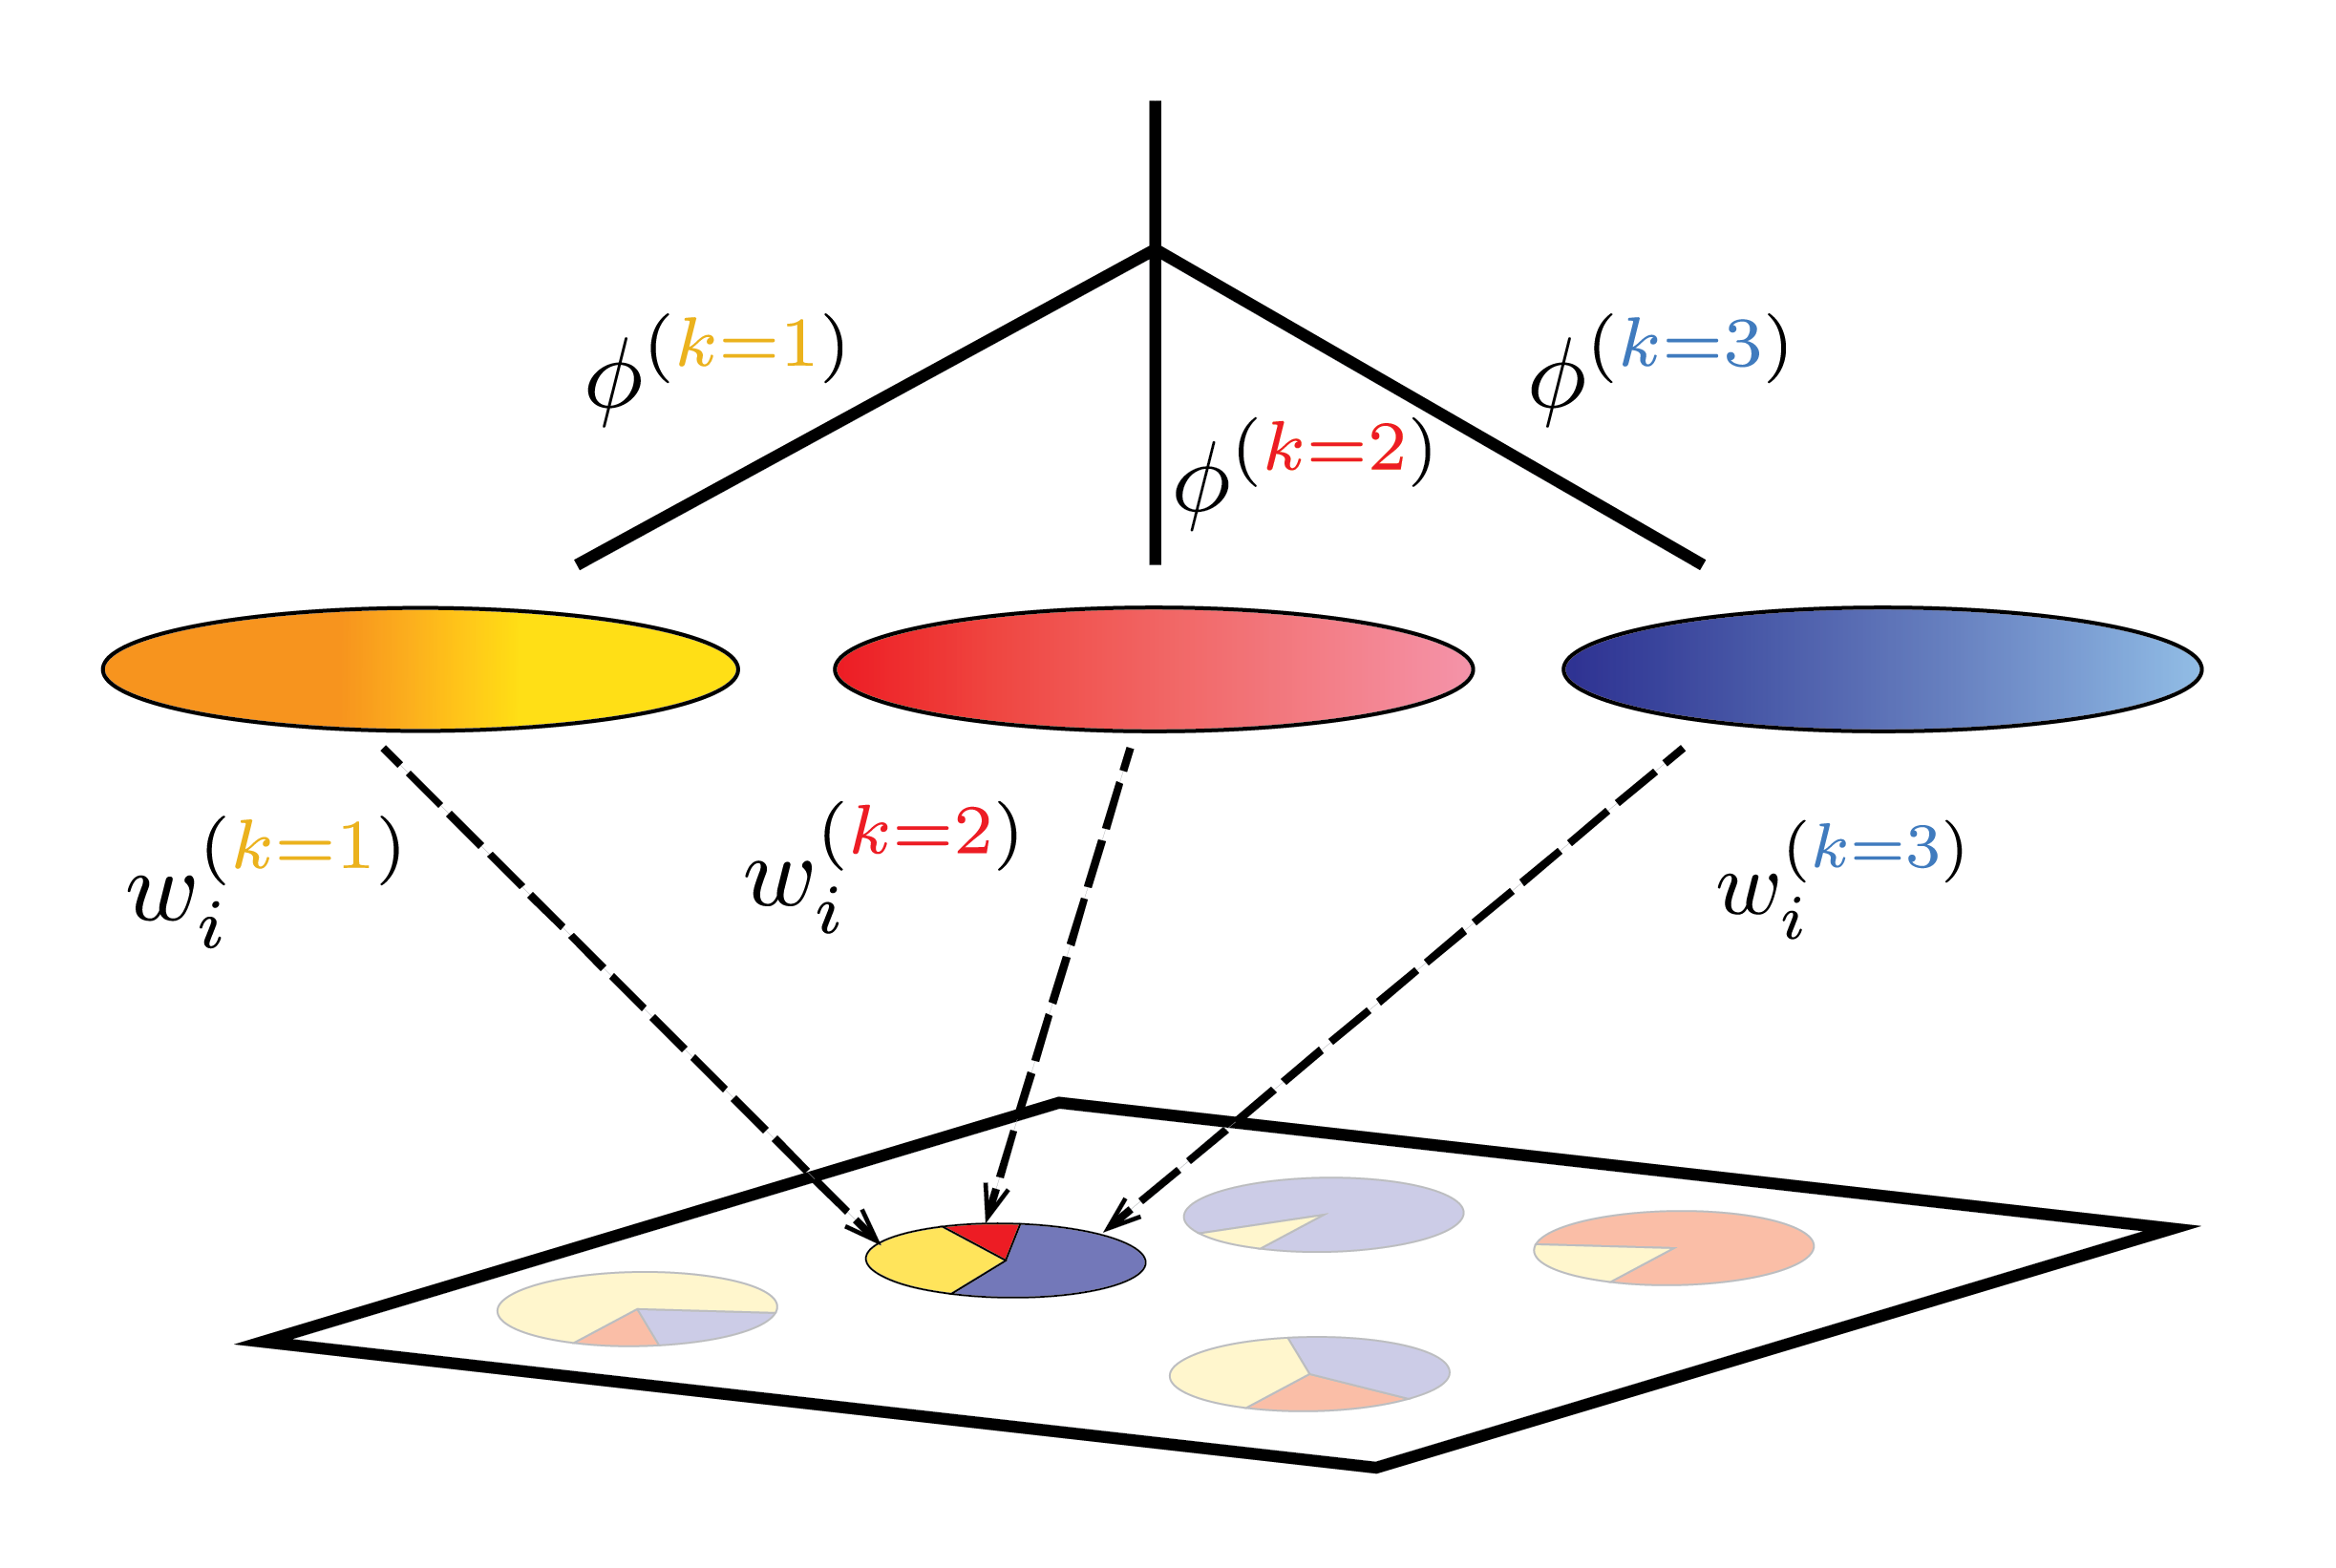
\includegraphics[width=4in,height=2.5in]{figs/schematic/method_schematic.png}}
		\caption{Schematic of our method, using $K=3$ as an example.
			     The pattern of isolation by distance within each layer is denoted by the color gradient in each of the layer ellipses, 
			     and $\phi_{(k)}$ denotes the covariance shared by samples with ancestry entirely in the $k$th cluster.
			     Sampled populations on the landscape are inferred to be admixed between these layers; 
			     the $i$th sample draws proportion $w^{(k)}_i$ of its ancestry from cluster $k$.
			    }\label{schematic}
\end{figure}

We can then describe the covariance between samples $i$ and $j$ across all layers, $\Omega_{i,j}$,
by summing their within-cluster spatial covariances ($G_{i,j}^{(k)}$ in cluster $k$) across all $K$ layers,
weighted by the relevant admixture proportions.
\begin{equation}
\Omega_{i,j} = \gamma + \sum\limits_K w^{(k)}_i w^{(k)}_j
G^{(k)}_{i,j} + \delta_{i,j}\eta_i .
\label{cross_cluster_covariance}
\end{equation}
In this equation, $w^{(k)}_i w^{(k)}_j$ is the proportion of alleles that \emph{both}
sample $i$ and sample $j$ have inherited from cluster $k$.

In addition to the admixture-weighted sum of the within-cluster spatial covariances,
this function contains two terms, $\gamma$ and $\delta_{i,j}\eta_i$.
The first, $\gamma$, describes the global allelic covariance between all samples, 
and arises because all samples share an ancestral mean allele frequency at each locus,
which generates a base-line covariance.
In the final term, $\delta_{i,j}$ is an indicator variable that takes a value of 1 when $i$ equals $j$ and 0 otherwise,
and $\eta_i$ adds variance specific to sample $i$.
This term on the diagonal of the parametric covariance matrix captures processes shaping variance within the sampled deme, 
such as inbreeding and the sampling process.

\paragraph{Likelihood and inference}
If allele frequencies at each locus
were independent between loci and multivariate normally distributed across populations, 
then their allelic covariance $\widehat{\Omega}$ 
would be Wishart distributed with degrees of freedom equal to $L$, 
the number of loci genotyped.
We use this as a convenient approximation to the true distribution described above,
and so define the likelihood of the allelic covariance to be
\begin{equation}
P(\widehat{\Omega} \; | \; \Omega) = \mathcal{W} \left( L\widehat{\Omega} \; | \; \Omega,L\right) .
\end{equation}
Linkage disequilibrium (LD) between loci will decrease the effective number of degrees of freedom, 
a complication we discuss further below.

We estimate the values of the parameters of the model using a Bayesian approach.
Acknowledging the dependence of the parametric covariance matrix $\Omega$ on its constituent parameters
$w,\alpha,\phi,\eta,\gamma$ and on the (observed) geographic distances $D$ 
with the notation $\Omega(w,\alpha,\phi,\eta,\gamma,D)$,
we denote the posterior probability density of the parameters as:
\begin{equation}
P\left( w,\alpha,\phi,\eta,\gamma \;	| \; \widehat{\Omega}, L \right) \propto
P\left(\widehat{\Omega} \; | \; \Omega(w,\alpha,\phi,\eta,\gamma,D) \right)
P(w)P(\alpha)P(\phi)P(\eta)P(\gamma) ,
\end{equation}
where $P(w)$, $P(\alpha)$, $P(\phi)$, $P(\eta)$, and $P(\gamma)$, are prior distributions.
All parameters are given (half-)Gaussian priors except for $\alpha_2$, which is uniform on $(0,2)$ and $w$, which is Dirichlet
(see Table \ref{tab:param_prior_tab} for specifics).
Parameters are independent between layers.
We use Hamiltonian Monte Carlo as implemented in STAN \citep{stan, NUTS, stan_lib, rstan} 
to estimate the posterior distribution on the parameters.
We also provide an R package \citep{R} called \texttt{conStruct} that functions as a wrapper 
around this inference machinery.


\paragraph{Relationship of this model to nonspatial structure models}

A nice feature of our approach is that the model described in Eqn \eqref{cross_cluster_covariance} 
contains a nonspatial assignment model as a special case 
(see \secref{model_app} for a more in-depth discussion). 
By setting $\alpha_0^{(k)}$ to zero for all $k$, 
we obtain a nonspatial model in which each cluster has its own allele frequency at each SNP, 
and individuals draw a proportion of their ancestry from each cluster. 
This model is strongly conceptually similar to that of STRUCTURE \citep{STRUCTURE} 
and related models \citep[e.g.][]{ADMIXTURE}; 
the only difference is that our likelihood assumes that allele frequencies are normally distributed 
around their expectations, 
while the standard assignment methods assume that the error is binomially distributed \citep{Engelhardt2012}.  
Therefore, we can compare the fit of the different models 
--- spatial vs. nonspatial, across different values of $K$ --- 
by comparing their performance in a common framework.

\paragraph{Choice of cluster number and cross-validation}
There are a number of reasons, both statistical and biological, 
why there is no true (or right) number of layers for real datasets,
discussed further in the Discussion.
However, it is still important to assess whether additional spatial layers (larger $K$)
meaningfully model patterns in the data
or merely explain spurious variation introduced by noise
-- in other words, whether additional model complexity
provides significant explanatory power.
Toward that end, we have implemented a method for 
statistically comparing \texttt{conStruct} results across different values of $K$ 
and between the spatial and nonspatial models.

Several approaches have been used as model choice criteria 
for the number of clusters in population genetic data, including: 
information theoretic criteria \citep[e.g.][]{ADMIXTURE}, such as AIC or BIC;
comparisons of the likelihood of the data across different values of $K$, 
with various criteria on how to choose a single value (e.g., \citep{Evanno2005});
or comparisons of the marginal likelihood, 
generated either via various approximations \citep[e.g.][]{STRUCTURE}
or via a more rigorous and computationally intensive approach such as thermodynamic integration \citep{verity_nichols2016}
or inference using a Dirichlet process prior \citep{huelsenbeck2007inference}.
See \cite{verity_nichols2016} for a discussion of these approaches and comparison
between several methods.

We use cross-validation \citep[similar in spirit to][]{ADMIXTURE_xval} to attack this problem.
To do this,
we use a ``training" partition of the data (in practice, a random 90\% subset of the loci)
to estimate the posterior distribution of the parameters,
and then calculate the log-likelihood of the remaining ``testing'' loci,
averaged over the posterior.
Prediction accuracy of a particular model (e.g., value of $K$)
is then measured using this log-likelihood,
averaged over a number of independent data partitions.
The best model is judged to be the simplest one with significantly better predictive accuracy
than others (see \secref{Xvalidation} for more on our cross-validation procedure).
In general, larger values of $K$ allows the model more flexibility,
and thus increases the likelihood of the training partition, 
but this improvement in the likelihood will plateau (or even peak), 
since above a certain $K$ the model only fits noise specific to the training data 
rather than generalizable patterns.
At any value of $K$, support for the spatial model over the nonspatial model 
means that isolation by distance is likely a feature of the data.

Cross-validation provides a valuable summary of how much explanatory power
is added by spatial structure within each layer, and each additional layer.
A simple $t$-test can be used to assess whether additional layers
show statistically significantly greater predictive accuracy.
However, we remind users that ``statistical significance does not imply real-world significance'',
and so small but statistically significant differences between models
should probably not be relied on too strongly.

An additional heuristic to evaluate the inclusion of additional layers is to calculate 
each layer's relative contribution to total covariance as their importance, 
and to choose a value of $K$ where all layers have an importance above some cutoff (e.g. 0.1\%).
Because the prior on admixture proportions is a Dirichlet distribution 
that is quite harsh against intermediate admixture values (see Table \ref{tab:param_prior_tab}),  
the model will tend to ``not use" unnecessary layers, 
and they will have a low contribution to overall covariance.
The contribution of the $k$th layer can be calculated as
its contribution to the parametric covariance between samples 
summed over the upper triangle (excluding the diagonal) of the covariance matrix.
The importance of the $k$th layer is its contribution relative to those of all other layers, 
i.e., its contribution divided by the sum of the contributions of all $K$ layers
(for details on calculating this importance, see Appendix \secref{layer_importance}). 
This layer importance is similar to the ``ancestry contribution'' proposed by \cite{fastStructure}. 
However, each of our layers can induce a different amount of covariance between samples embedded in them, 
so we take that into account when calculating each layer's contribution to the whole.

\section*{Results}

\subsection*{Simulations}
We first test the method with scenarios generated using the coalescent simulator \texttt{ms} \citep{Hudson2002}.
To generate discrete population structure, we simulate $K$ distinct populations,
each of which split from a common ancestor $\tau_{\text{s}}$ units of coalescent time in the past,
without subsequent migration between them.
To generate continuous differentiation within each cluster,
at time $\tau_{\text{e}}$ in the past,
each of these discrete clusters instantaneously colonizes a lattice of demes,
for which we use a stepping stone model with symmetric migration 
to nearest neighbors (eight neighbors, including diagonals).
Finally, at time $\tau_{\text{a}}$ in the past 
we generate a single dataset 
by collapsing those $K$ discrete lattices into a single grid of demes that are admixed to various degrees from these different layers.
(see Fig \ref{sim_setup}).
We simulated datasets using $K=1$, 2, and 3 layers,
in each sampling 10,000 unlinked loci from each of 20 haploid individuals from every deme.

We ran \texttt{conStruct} analyses on each of these simulated datasets, 
specifying both a spatial and nonspatial model for $K = $ 1 through 7, 
then used cross-validation to compare the predictive performance of the models.
In Fig \ref{simK1_pies}, we show the results of the analyses of the dataset simulated under $K=1$, 
contrasting the results of the nonspatial model runs with 2 - 4 clusters 
with those of spatial model with 2 - 4 layers.
In Fig \ref{sim_xvals} we show the results of the cross-validation analysis for each of the three simulated datasets.
The results of all analyses run on datasets simulated using $K=1$ through 3 are shown in 
Figs \ref{simK1_nsp_pies}-\ref{simK3_adprop_fit}.
To confirm that results from our nonspatial model were qualitatively similar to those of 
other nonspatial model-based clustering algorithms, 
we also analyzed each simulated dataset using fastSTRUCTURE \citep{fastStructure}, 
inferring admixture under models with $K=2$ through 4 (Figs \ref{fastStr_simK1}-\ref{fastStr_simK3}).

A number of results are immediately clear from these tests with simulated data.
First, \texttt{conStruct} performs well on all simulated scenarios.
Across all values of K and for all simulations, 
the spatial model is correctly preferred over the nonspatial model (Fig \ref{sim_xvals})., 
and it infers the true admixture proportions with high accuracy, tight precision, and good coverage 
(Figs \ref{simK2_adprop_fit} and \ref{simK3_adprop_fit}).
Second, the predictive accuracy of the nonspatial model increases 
with the number of clusters in the model, 
as it describes continuous, spatial patterns of relatedness between demes within the same cluster 
using gradients of admixture across more and more discrete clusters.
This behavior of the nonspatial model is highlighted in 
the analyses of data simulated under $K=1$ (Fig \ref{simK1_pies} and \ref{simK1_nsp_pies}):
as $K$ in the model increases, 
the sampled area is increasingly divvied up between clusters 
with ``centers of mass" in the $K$ geographical extremes of the simulated space.
At $K=2$, the clusters are centered in opposite corners on the map; 
at $K=3$, in the lower two corners and the top half; 
at $K=4$, all four corners, and so on.
These results are qualitatively similar to those generated using fastSTRUCTURE \citep{fastStructure}, 
which also describes continuous differentiation using admixture between clusters
 (Fig \ref{fastStr_simK1}-\ref{fastStr_simK3}).
While it is true that each cluster is more similar within itself
than it is to other clusters,
we know that these boundaries are arbitrary,
since the data were simulated with no such boundaries.

In contrast, the predictive accuracy of the spatial \texttt{conStruct} model
either plateaus at or declines from the true value of $K$ used to simulate the data 
(Figs \ref{sim_xvals}, \ref{simK1_xval}, \ref{simK2_xval}, and \ref{simK3_xval}).
And, as $K$ in the spatial model increases, 
deme membership in layers beyond the number used to simulate the data does not appreciably increase 
(Fig \ref{simK1_sp_pies}, \ref{simK2_sp_pies}, \ref{simK3_sp_pies}).
That is, even when the spatial model is run with $K=7$, 
the inferred admixture proportions are nearly identical to 
those estimated under the true value of $K$ for each simulation.
These results are highlighted in the calculation of layer importance for 
analyses run in each simulation (Fig \ref{simK1_laycon}, \ref{simK2_laycon}, and \ref{simK3_laycon}).
In the spatial analyses run using the true value of $K$,
the importance of the $K$ layers remains constant even with additional layers;
in contrast, additional layers in the nonspatial analyses continue to be important for describing variation.

\begin{figure}
	\centering
		\subcaptionbox{$K=2$\label{simK1_pies:nsp_K2}}
			{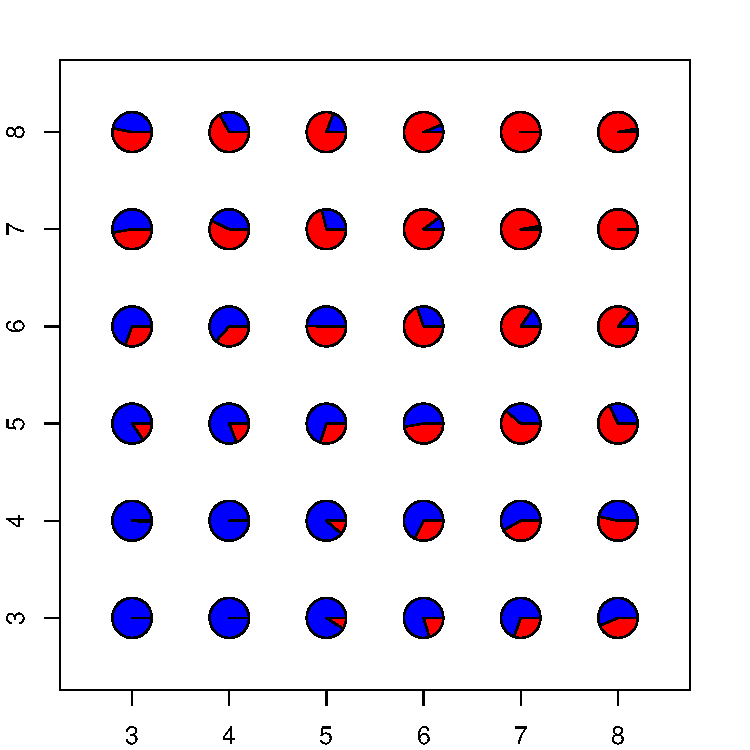
\includegraphics[width=1.8in,height=1.8in]{figs/sims/simK1_nsp_pies_K2.pdf}}
		\subcaptionbox{$K=3$\label{simK1_pies:nsp_K3}}
			{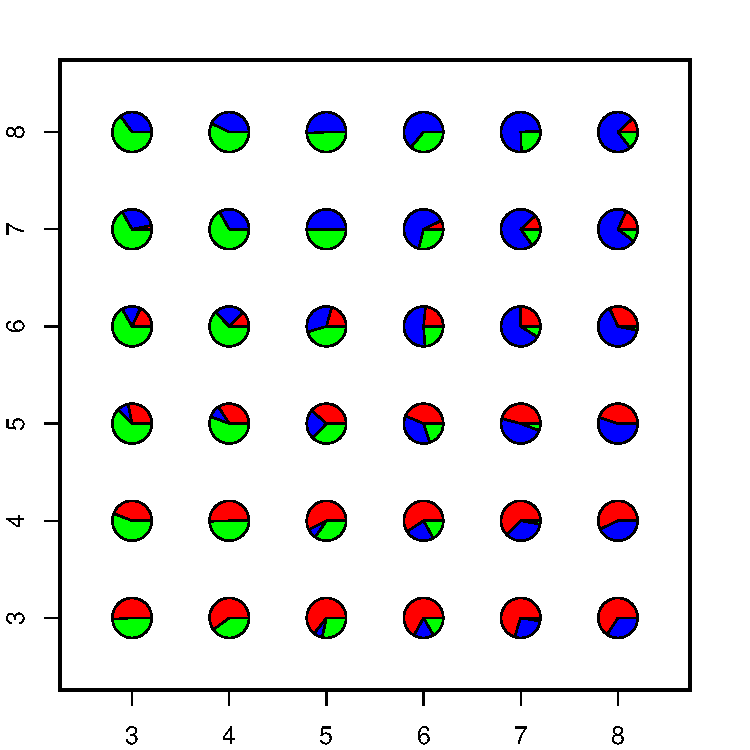
\includegraphics[width=1.8in,height=1.8in]{figs/sims/simK1_nsp_pies_K3.pdf}}
		\subcaptionbox{$K=4$\label{simK1_pies:nsp_K4}}
			{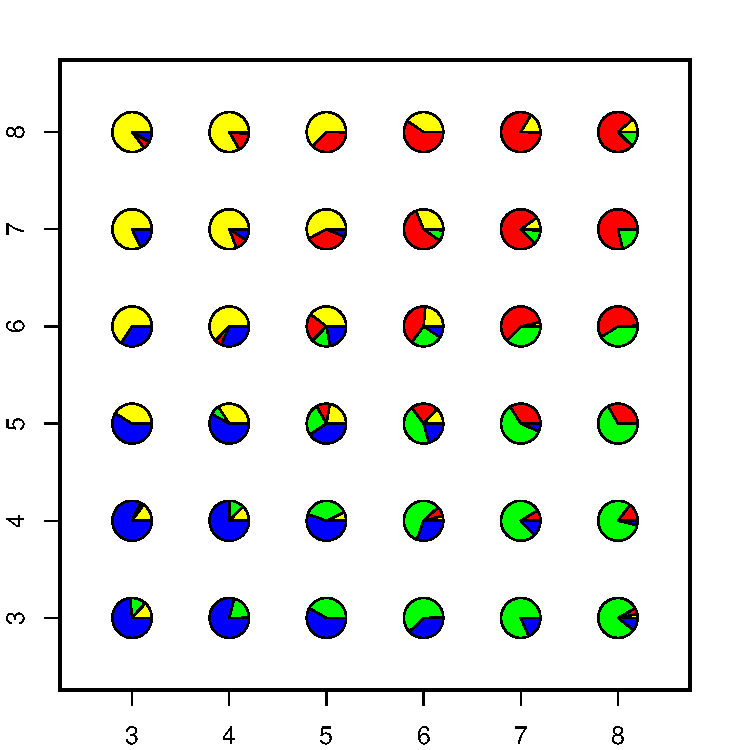
\includegraphics[width=1.8in,height=1.8in]{figs/sims/simK1_nsp_pies_K4.pdf}}
		\subcaptionbox{$K=2$\label{simK1_pies:sp_K2}}
			{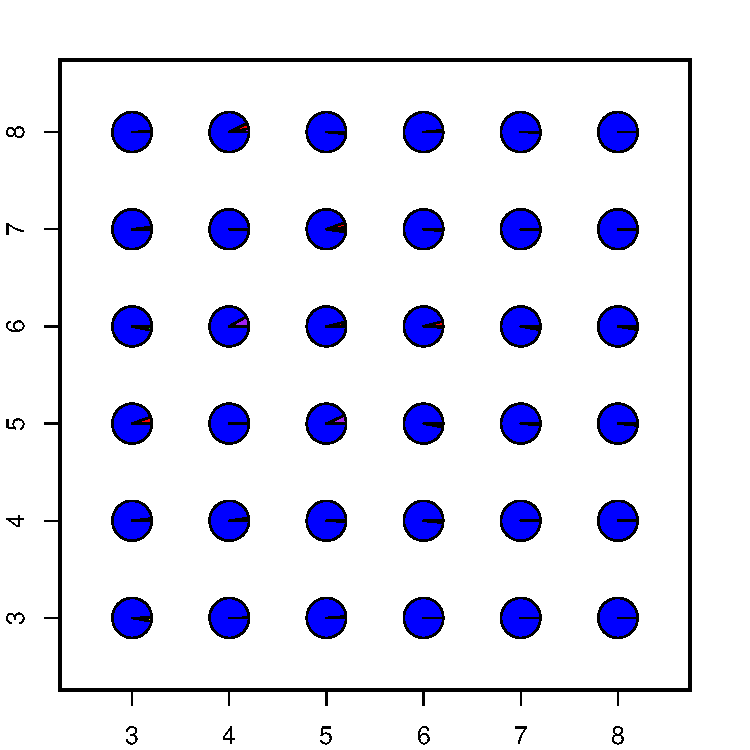
\includegraphics[width=1.8in,height=1.8in]{figs/sims/simK1_sp_pies_K5.pdf}}
		\subcaptionbox{$K=3$\label{simK1_pies:sp_K3}}
			{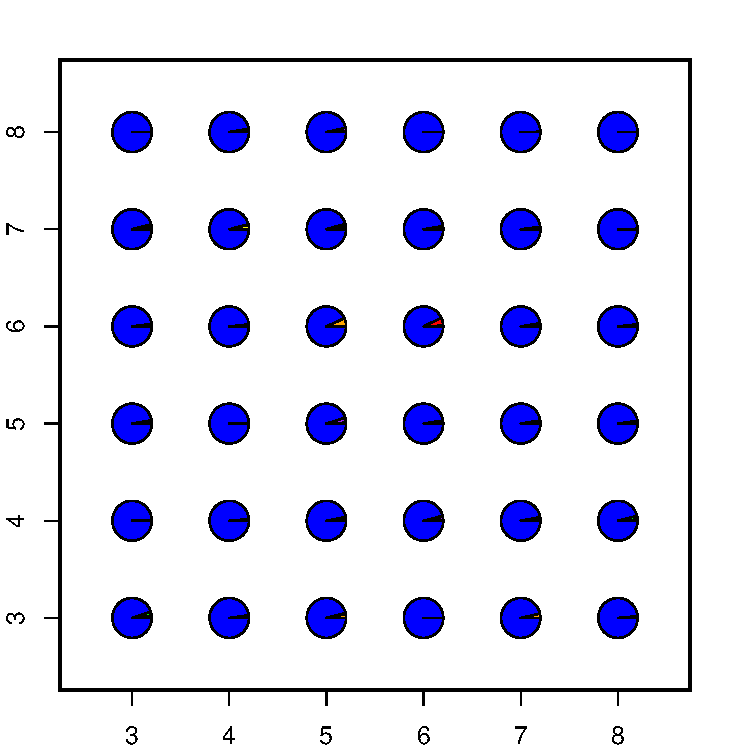
\includegraphics[width=1.8in,height=1.8in]{figs/sims/simK1_sp_pies_K6.pdf}}
		\subcaptionbox{$K=4$\label{simK1_pies:sp_K4}}
			{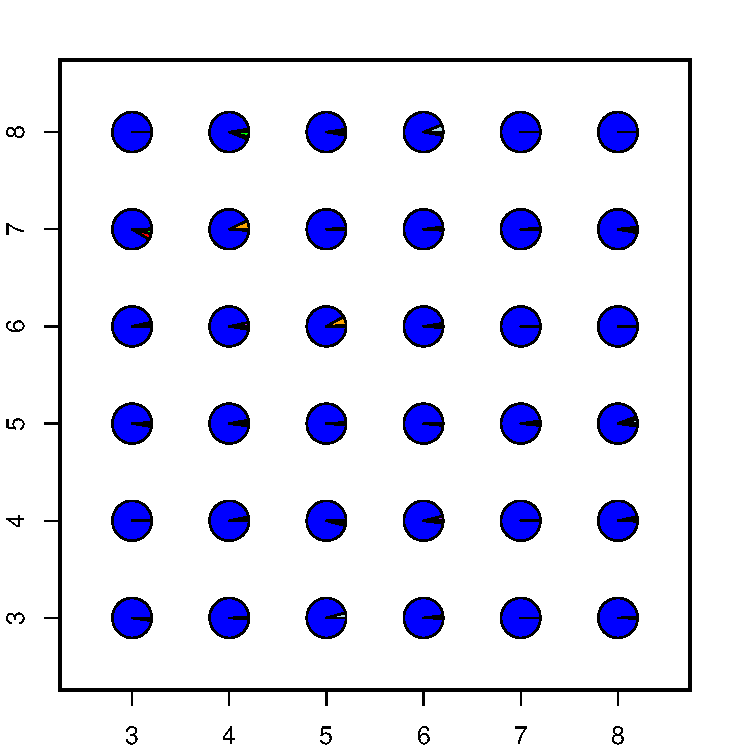
\includegraphics[width=1.8in,height=1.8in]{figs/sims/simK1_sp_pies_K7.pdf}}
	\caption{
	Map of admixture proportions estimated using the nonspatial model for $K=2$ through 4 (top row)
	and also the spatial model for $K=2$ through 4 (bottom row).
	The data were simulated using a single cluster with nearest-neighbor symmetric migration between demes.
    }\label{simK1_pies}
\end{figure}

\begin{figure}
	\centering
		{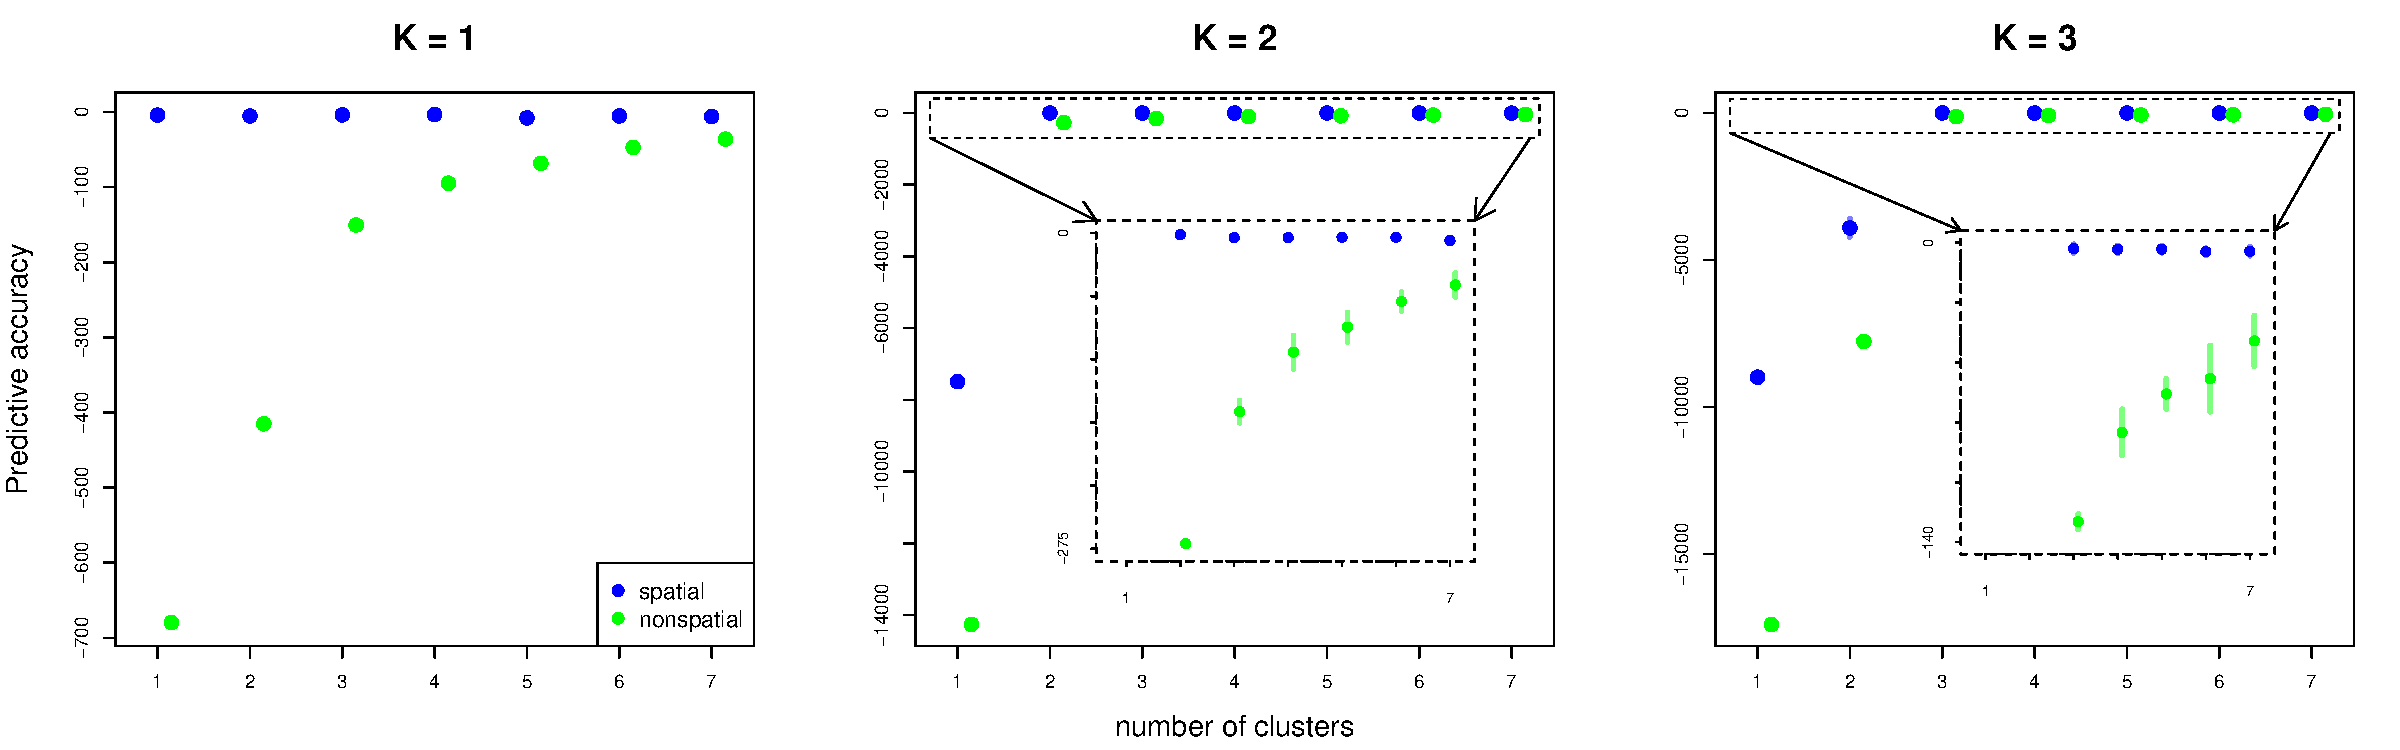
\includegraphics[width=6in,height=2in]{figs/sims/sim_xvals.pdf}}
	\caption{
	Cross-validation results for data simulated under $K=1$, $K=2$, and $K=3$, 
	comparing the spatial and nonspatial \texttt{conStruct} models run with $K=1$ through 7.  
	The inset plots zoom in on cross-validation results outlined in the dotted boxes.
    }\label{sim_xvals}
\end{figure}

\subsection*{Empirical Applications}
To demonstrate the utility of this method, we analyzed empirical population genomic data from two systems:
a contact zone between two poplar species in northwestern North America,
and a large North American sample of black bears.

\subsubsection*{Poplars}

Trees in the genus \textit{Populus} (poplars, aspens, and cottonwoods) 
are distributed throughout the Northern Hemisphere;
species in the genus regularly co-occur and, 
where they do, they frequently hybridize \citep{eckenwalder1984, Cronk2005}.

Here, we focus on two \textit{Populus} species in the Pacific Northwest: 
\textit{Populus trichocarpa}, the black cottonwood,
and \textit{Populus balsamifera}, the balsam poplar.
These species have a broad zone of overlap and are hypothesized to hybridize \citep{geraldes_etal_2014, suarezgonzalez_etal_2016}.
Both species are sampled over a large geographic region, 
and show spatial patterns of genetic and phenotypic variation \citep{slavov_etal_2012, mckown_etal_2013},
making the system well-suited to test an analysis designed to describe
how genetic structure is partitioned both discretely across population (or species) clusters
and continuously with geographic distance.
We organize the results of our analyses around the following questions: 
\begin{enumerate}
\item Given the known history of hybridization between this pair of poplar species, 
is there support for two discrete clusters, 
rather than a single cline of ancestry across their overlap zone?
\item If there is evidence for discrete population structuring, 
does it fall solely along species boundaries, 
or is there sub-structuring between different populations of the same species?
\item Is there support for a pattern of isolation by distance within
the inferred clusters, and, if so, 
does it differ between different layers?
\end{enumerate}

Our data, originally published by \cite{geraldes_etal_2014}, 
consist of 434 individuals sampled from 35 drainages 
and genotyped at just over 33,000 loci (map of the sampling shown in Fig \ref{populus_map}).
The data were generated using RAD-seq, 
and showed a strong pattern of bias in allelic dropout 
(the majority of missing data were from drainages with only \textit{Populus balsamifera} individuals).
To ameliorate some of the problems that arise when there is a strong bias in which data are missing, 
we dropped loci for which any data were missing, 
resulting in just over 20,200 loci retained for analysis.  
We then analyzed these data, grouped by drainage, using both the spatial and nonspatial \texttt{conStruct} models, 
using $K = 1$ through 7,
and compared these models using cross-validation.
The results of these analyses are shown in 
Figs \ref{populus_xvals} and \ref{populus_pies}, 
as well as in Figs \ref{populus_sp_pies} - \ref{populus_laycon} in the Supplementary Materials.

\begin{figure}
	\centering
		\subcaptionbox{$K=2$\label{populus_pies:K2}}
			{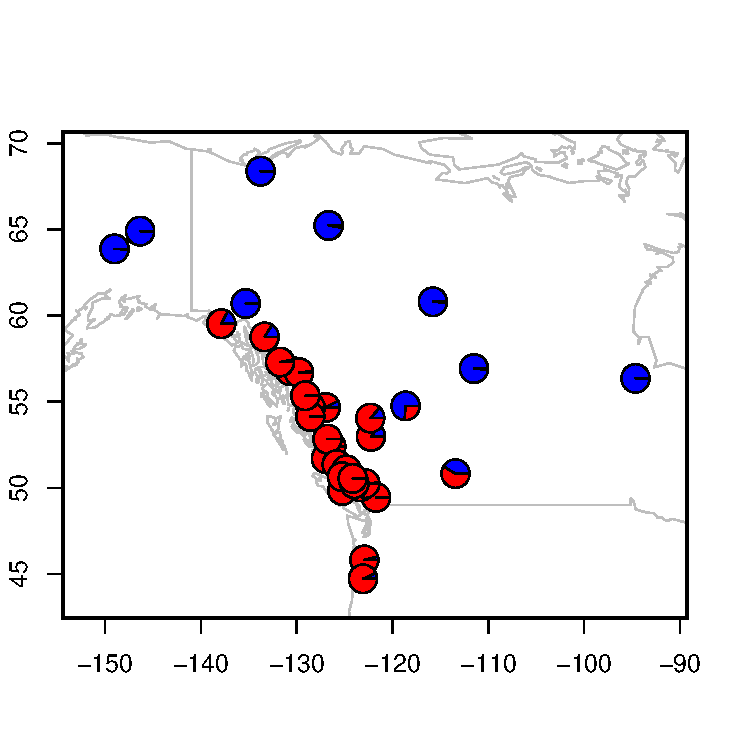
\includegraphics[width=1.8in,height=1.8in]{figs/populus/populus_sp2.pdf}}
		\subcaptionbox{$K=3$\label{populus_pies:K3}}
			{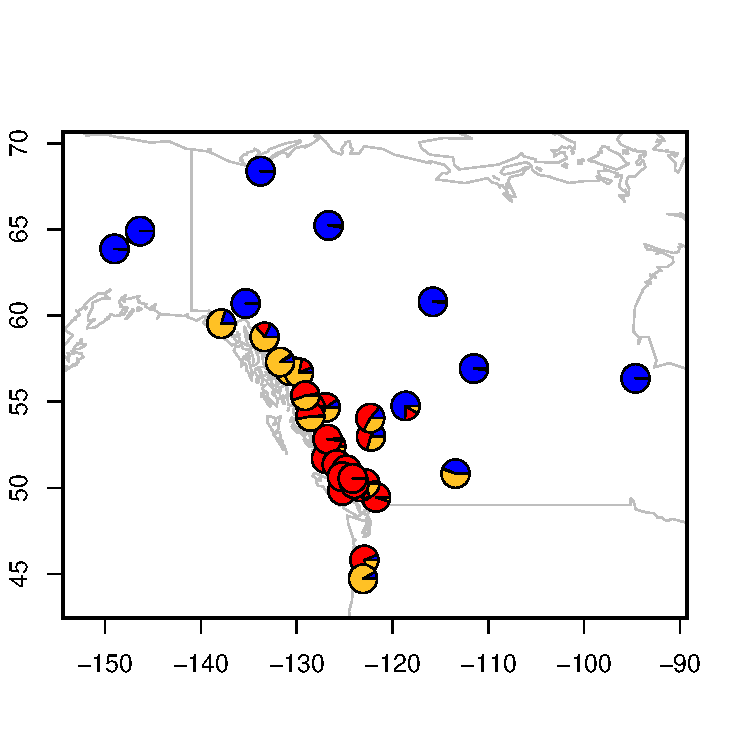
\includegraphics[width=1.8in,height=1.8in]{figs/populus/populus_sp3.pdf}}
		\subcaptionbox{$K=4$\label{populus_pies:K4}}
			{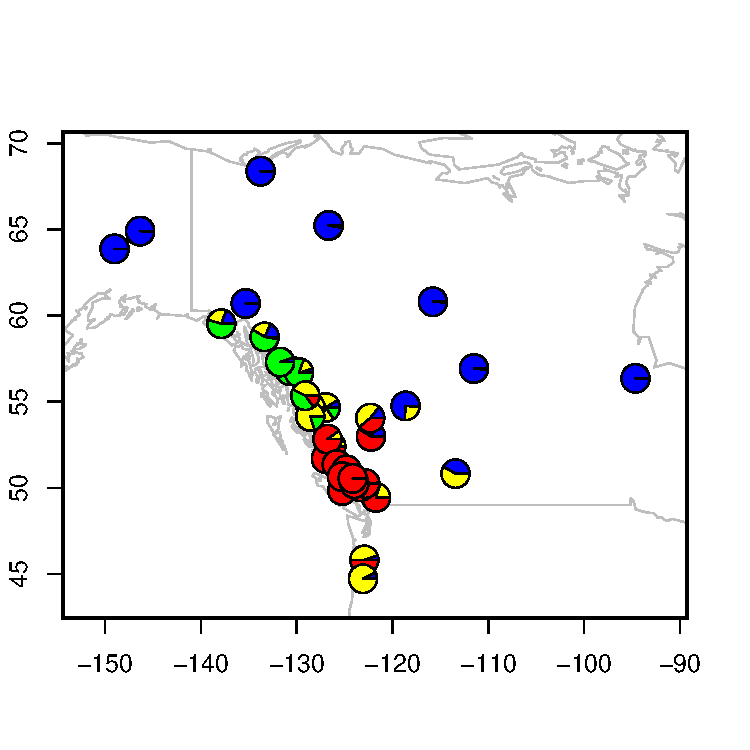
\includegraphics[width=1.8in,height=1.8in]{figs/populus/populus_sp4.pdf}}
	\caption{
	Map of admixture proportions estimated for the \textit{Populus} dataset 
	using the spatial model for $K=2$ through 4.
    }\label{populus_pies}
\end{figure}

\begin{figure}
	\centering
		{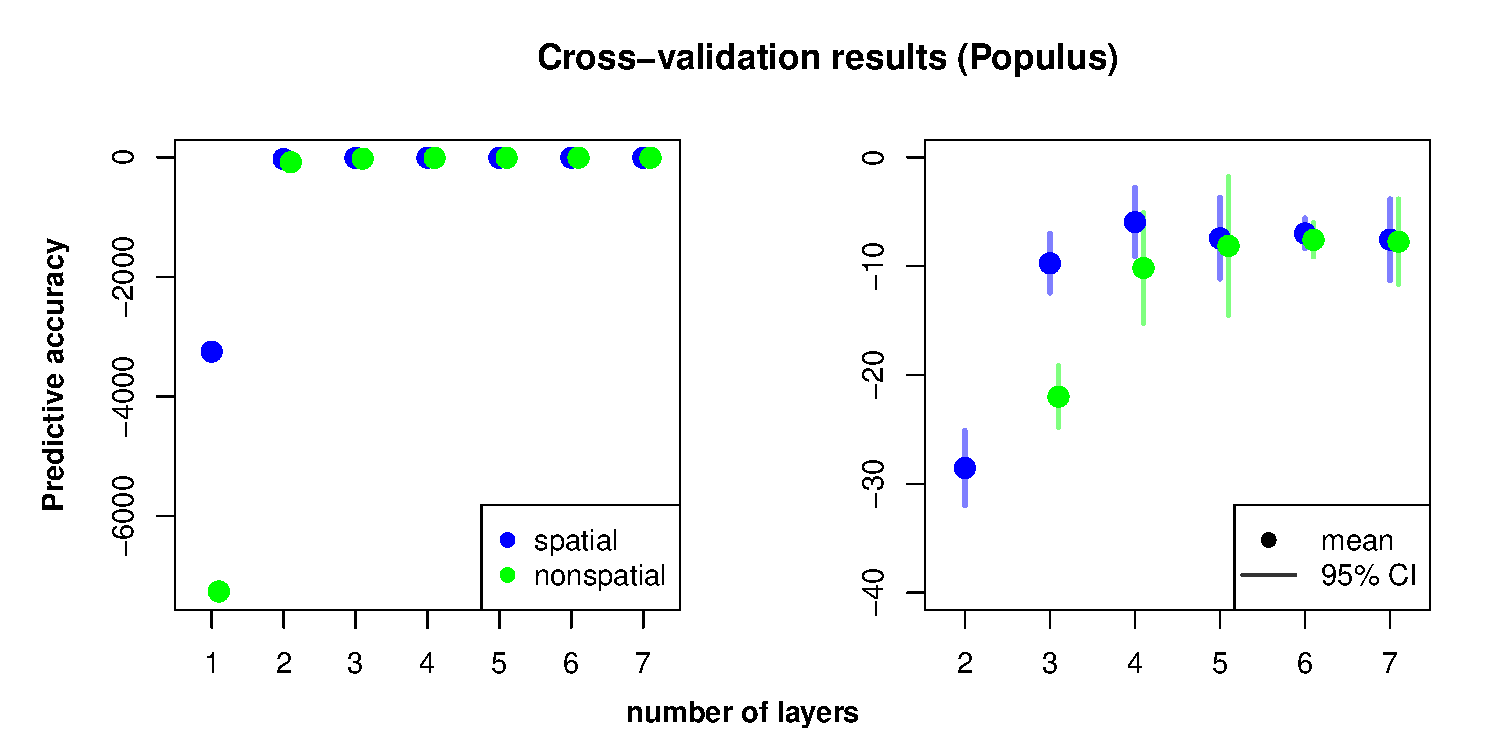
\includegraphics[width=6in,height=3in]{figs/populus/populus_std_xval.pdf}}
	\caption{
	Cross-validation results for \textit{Populus} dataset 
	comparing the spatial and nonspatial \texttt{conStruct} models run with $K=1$ through 7.  
	The first panel in each row shows all results; 
	the second panel zooms in on the results from analyses run with $K = 2$ through 7.
    }\label{populus_xvals}
\end{figure}

All models with $K>1$ assigned the majority of each species
to distinct layers, with some populations drawing ancestry from both layers.
This provides strong support for discrete population structure between the two species,
with some admixture,
rather than a single, continuous cline of ancestry.
At all values of $K>1$, discrete population structure was mostly partitioned along species lines; 
at values of $K$ above 2, further discrete substructure was inferred within the \textit{P. trichocarpa} samples, 
while \bals{} samples displayed no substructure up to $K=7$.
This lack of substructure within the sampled \bals{} populations is in agreement with results from 
\citet{keller_etal_2010}, who found that \bals{} in the region is characterized by relatively low diversity, 
and probably represents a recent, postglacial expansion.

A consistent split between layers within \tri{} fell along the ``no-cottonwood belt," 
a region along the central coast of British Columbia in which black cottonwood is absent. 
The no-cottonwood belt is hypothesized to divide the species' distribution 
into northern and southern groups, which, in a provenance test, 
were experimentally shown to display different phenotypes 
\citep[e.g., pathogen resistance,][]{xie2009,xie2012}.  
At higher values of $K$, drainages at the southern tip of \tri{} sampling 
begin to split out into their own layers.  
This may potentially be the result of introgression from southern \textit{Populus} species, 
such as \textit{P. angustifolia} or \textit{fremontii} \citep{Zhou2012,geraldes_etal_2014}

At all values of $K$, the spatial model was preferred over the nonspatial model (Fig \ref{populus_xvals}).
Most of this signal seems to derive from the \textit{P. trichocarpa} samples:
covariance within predominantly \tri{} layers decays more quickly with distance
than within the majority \bals{} layer, as seen in Fig \ref{populus_sp_clst_covs}.  
This indicates that, although isolation by distance is a feature of the dataset as a whole, 
it's magnitude varies considerably across biological units - 
an aspect of the data \texttt{conStruct} is able capture well.


\subsubsection*{Black bears}
The American black bear, \textit{Ursus americanus}, is endemic to North America
and has a broad distribution across the continent.
During the last glacial maximum, 
black bears were confined to isolated glacial refugia, 
from which they subsequently expanded to occupy their current range
\citep{WoodingWard1997,Byun1997,Stone2000,Puckett2015}.
The retreat of the glaciers was relatively recent in units of 
black bear generation times \citep{Onorato2004}, 
so we might reasonably expect the divergence accrued between refugia 
to be reflected in discrete genetic structure between extant populations.
Black bears are strong dispersers \citep{Moore2014}, 
but they are distributed across most of the continent, 
so we may therefore expect them to experience distance-limited 
mating opportunities and exhibit a pattern of IBD.
As with the poplars described above, 
this system is likely to present patterns of genetic structure 
that are both continuous and discrete, 
making it well-suited as a test for our method.
We organize the results of our analyses of 
the complicated landscape of genetic structure in black bears 
around the following questions:
\begin{enumerate}
\item How many historical clusters are reflected in modern patterns of genetic variation?
\item Do we see support for a pattern of isolation by distance within each of the inferred discrete groups?
\end{enumerate}

Our data, originally published by \cite{Puckett2015}, consist of 95 individuals 
sampled across the United States and on the West coast of Canada,
genotyped at just under 22,000 bi-allelic loci.
The distribution of missing data across these individuals was uneven, 
with a few individuals representing most of the missing data, 
so we removed individuals with greater than 4\% missing data, 
resulting in a final dataset of 78 individuals.
We then analyzed these data, treating individuals as the unit of analysis, 
using both the spatial and nonspatial \texttt{conStruct} models with a $K$ of between 1 and 7, 
and compared these models using cross-validation.
The results of these analyses are shown in Figs \ref{bear_xvals} - \ref{bear_laycon}, 
as well as in Figs \ref{bear_sp_pies} - \ref{bear_nsp_clst_covs} in the Supplementary Materials.

\begin{figure}
	\centering
		\subcaptionbox{$K=3$ (spatial)\label{bear_K3:sp}}
			{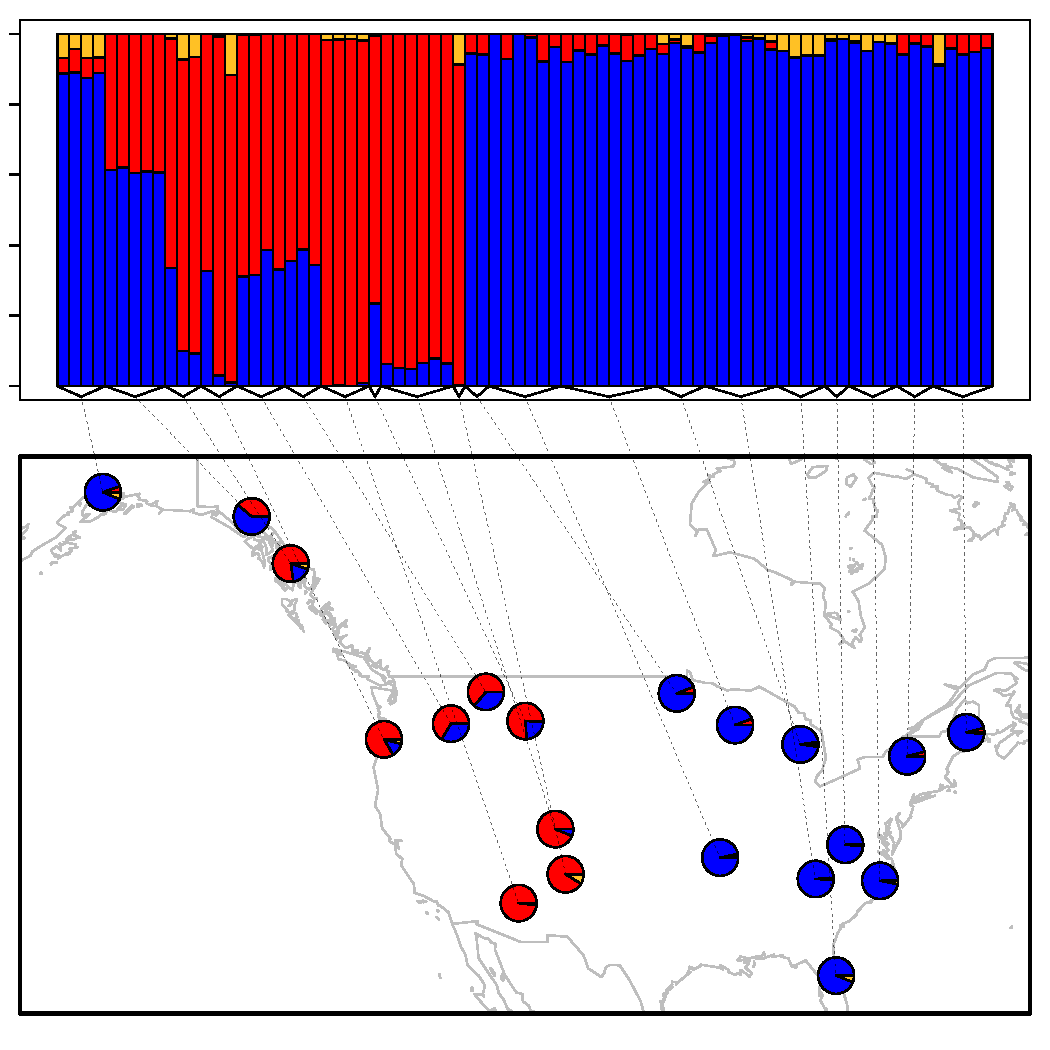
\includegraphics[width=2.5in,height=2.5in]{figs/bears/bear_sp3.pdf}}
		\subcaptionbox{$K=3$ (nonspatial)\label{bear_K3:nsp}}
			{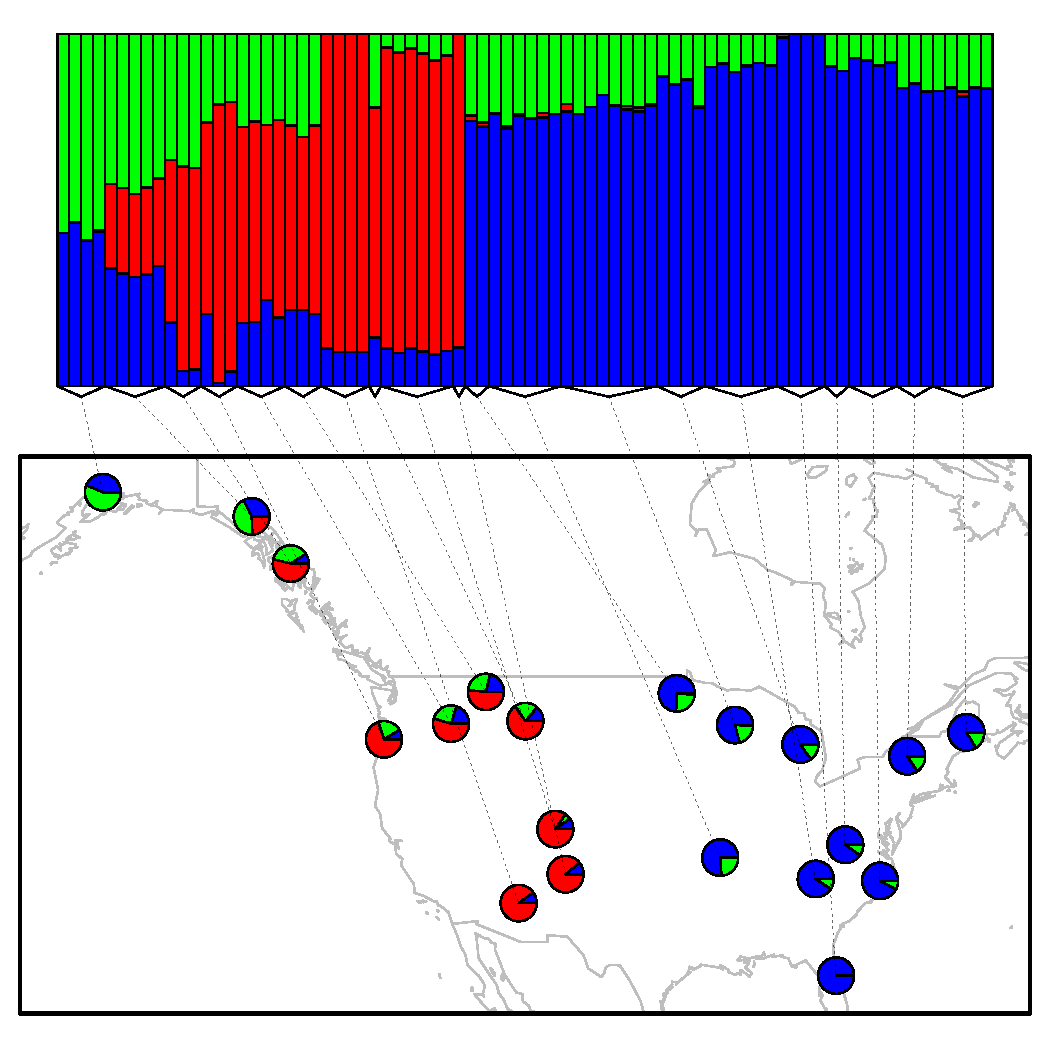
\includegraphics[width=2.5in,height=2.5in]{figs/bears/bear_nsp3.pdf}}
	\caption{
	Map sof admixture proportions estimated for the black bear dataset 
	using the spatial model (left) and the nonspatial model (right) for $K=3$.
	Pies show mean admixture results across individuals within their diameter, 
	and the admixture results for all individuals included within each group are 
	shown in the plot above.
    }\label{bear_K3}
\end{figure}

\begin{figure}
	\centering
		{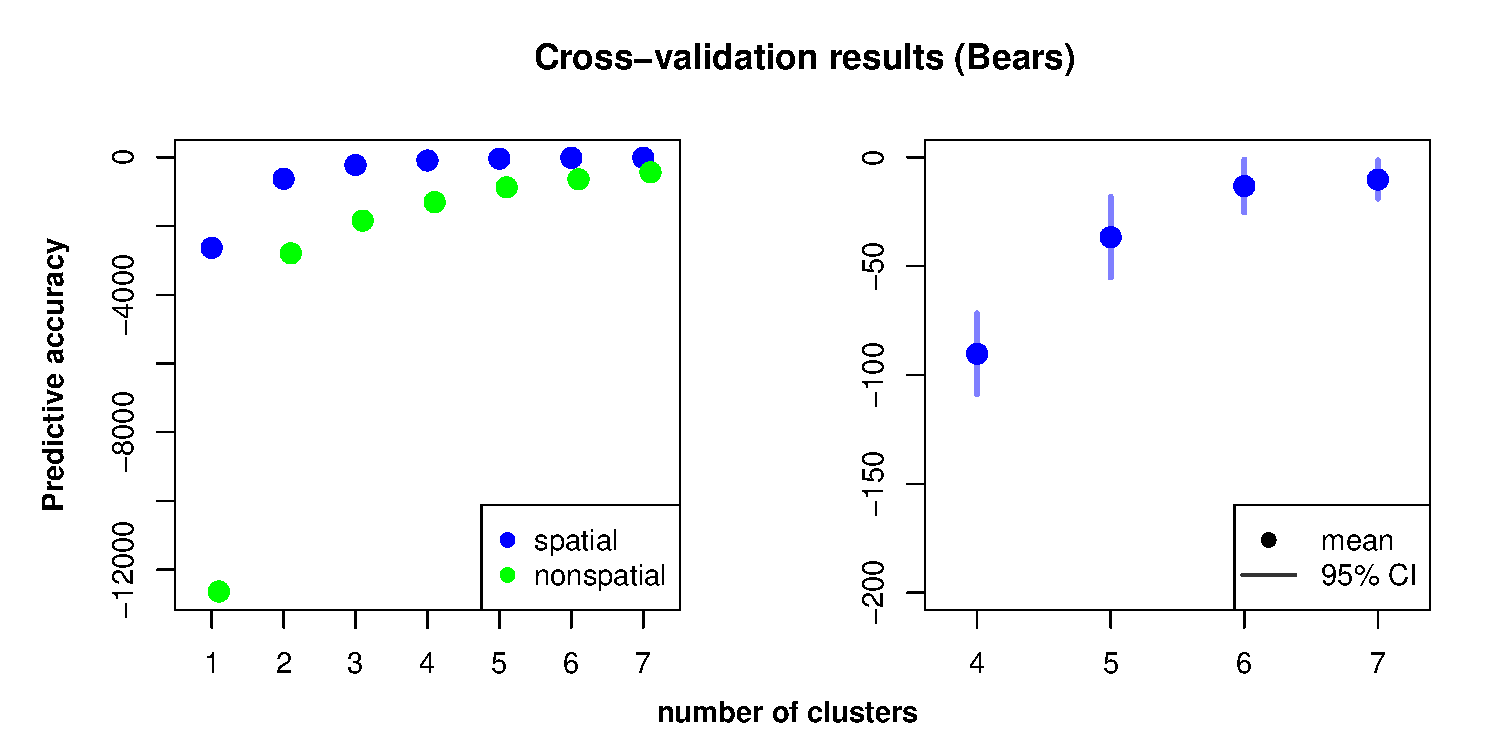
\includegraphics[width=6in,height=3in]{figs/bears/bear_std_xval.pdf}}
	\caption{
	Cross-validation results for black bear dataset 
	comparing the spatial and nonspatial \texttt{conStruct} models run with $K=1$ through 7.  
	The first panel in each row shows all results; 
	the second panel zooms in on the results from the spatial analyses run with $K = 4$ through 7.
    }\label{bear_xvals}
\end{figure}

\begin{figure}
	\centering
		{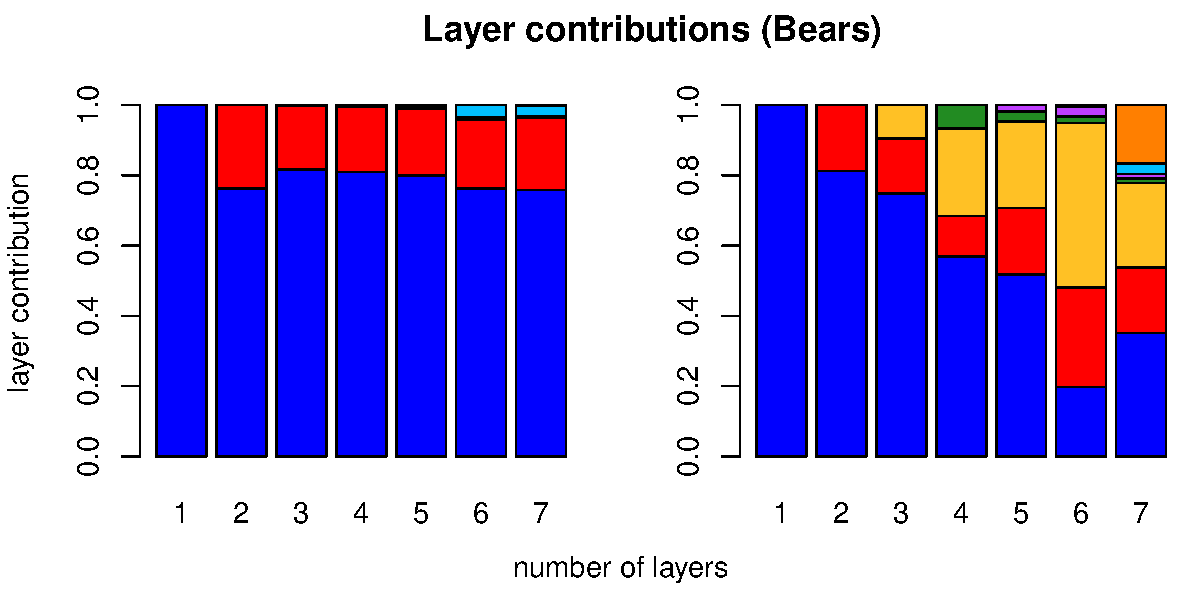
\includegraphics[width=6in,height=3in]{figs/bears/bears_laycon_barplots.pdf}}
	\caption{
	Layer ``contributions" (i.e., how much total covariance is contributed by each layer), 
	for all layers estimated in runs using $K = 1$ through 7 
	for the spatial model (left) and the nonspatial model (right).
	For each value of $K$ along the x-axis, there are an equal number of layer contributions plotted.
	Colors are consistent with Fig \ref{bear_K3}.
    }\label{bear_laycon}
\end{figure}

Bears in the sample are partitioned into two main groups:
one to the east of the Rocky Mountains, 
which also occurs in Alaska, and, presumably, 
in the intervening (unsampled) northern Great Plains and Canadian Shield;
the other primarily west of the Rockies, 
but presumably stretching up into British Columbia.
Additional layers in the spatial model have strong statistical support 
up until around $K=5$ or 6 (Fig \ref{bear_xvals}).
However, upon examining layer importance (Fig \ref{bear_laycon}),
it is clear that the additional layers beyond $K=2$ are contributing only a very small amount toward 
total covariance between individuals.
The locations of the individuals inferred to be admixed between the two layers 
provide information about a possible zone of contact and migration between these groups 
along the northwestern coast of North America and near the Cascade Range in the northern U.S.
These findings are consistent with a scenario of postglacial expansion from two refugia, 
one in the American Southwest and one in the American Southeast, 
but lack of any samples from Canada and Mexico, 
and lack of denser sampling across northern North America, 
make more detailed interpretations untrustworthy.
In addition, our model is not an explicit test of any demographic scenario, 
and also uses a dataset that consists solely of nuclear (rather than mitochondrial) DNA.

Results from the nonspatial model clearly exhibit the tendency 
of nonspatial clustering algorithms to describe continuous spatial patterns of divergence 
using gradients of admixture between clusters.
For example, in Fig \ref{bear_K3:nsp}, 
the third cluster (in green) exhibits a clear East-West gradient that 
is overlain across the discrete structure between the Southwest cluster and the Southeast 

Across all values of $K$ for which we ran \texttt{conStruct},
we see strong support for the spatial model over the nonspatial model (Fig \ref{bear_xvals}),
indicating the isolation by distance seems to be a prominent feature of the data.
This pattern may resolve a discrepancy between our results and 
previous analyses that split Alaskan and British Columbian bears out 
into their own cluster with an inferred Beringian glacial refugium
\citep{Byun1997,Stone2000,Puckett2015}.
Our model, which explicitly incorporates a spatial decay of relatedness, 
allows individuals sampled at a large remove to belong to the same layer
instead of splitting these individuals out into successive clusters.

%%%%%%%%%
\section*{Discussion}

The pattern of isolation by distance is ubiquitous in nature;
this is unsurprising, as mating opportunities are distance-limited in most species.
This common pattern can flummox commonly used clustering methods, 
which must use a possibly large number of discrete clusters
to describe such continuous population differentiation.
Inference of these spurious clusters can have implications for 
downstream analysis and interpretation of genetic data, 
including conservation management decisions and 
identification of the genetic basis of adaptation or disease traits.

In this paper, we have presented a statistical framework, \texttt{conStruct}, for simultaneously 
modeling continuous and discrete patterns of population structure.
By employing the sensible default assumption
that relatedness ought to decay with distance, even within a population, 
we avoid erroneously ascribing population differentiation to discrete population clusters.
We also present a cross-validation approach for comparing between models, 
although we stress the limits of this or any model selection procedure for genetic clustering.

The method performs well on simulated data:
we accurately infer the admixture proportions used to simulate the data 
and accurately pick the simulating model as the best model using our cross-validation procedure.
Empirical applications of \texttt{conStruct} to a sample of North American poplars 
and a sample of North American black bears yield reasonable results.

The proposed method combines the utility of model-based clustering algorithms 
with a biologically realistic model of isolation by distance.
We anticipate that \texttt{conStruct} will be useful for identifying populations 
and determining samples' ancestry in and across them, 
especially when the populations exhibit spatial patterns of relatedness.

\paragraph{Comparison to nonspatial model-based clustering}
Above, we showed that 
(a) the nonspatial \texttt{conStruct} model recapitulates results of 
other, commonly-used nonspatial clustering methods,
and 
(b) \texttt{conStruct} can concisely capture spatial structure, which is nearly always expected within clusters.
Given this, when should methods without spatial capability be used?
One advantage these have over \texttt{conStruct} is speed.
Although \texttt{conStruct}'s computation time is invariant 
with the number of loci included in the dataset 
(after the initial calculation of the allelic covariance), 
it scales poorly with number of samples.
The computationally limiting step is the inversion of the parametric covariance, 
which is an operation of order $O(n^3)$, 
whereas computation time for, e.g., STRUCTURE, 
scales linearly with number of samples. \gb{is this true?}
The other main difference is the model of noise,
but it is unclear what effects this may have,
or indeed, which is closer to the truth.

\paragraph{Choosing the ``best" number of clusters}
Although we recognize the utility of choosing a single, ``best'' value of $K$, 
and using only that analysis to communicate results, 
we want to emphasize that there are both statistical and biological reasons 
why there is no true best value of $K$.
From a statistical perspective, the choice of best $K$ is always relative to the data in hand.
This means both that sampling different individuals or loci 
from the same populations may yield a different ``best" $K$, 
but also 
-- unless the data were generated under the model itself --
that the support for larger values of $K$ is likely to increase with increasing amounts of data
(although perhaps only logarithmically).
In the limit of infinite data, the best value of $K$ 
may be the number of individuals included in the dataset.
From a biological perspective, 
it is important to stress that patterns of relatedness between individuals and populations 
are shaped by complex spatial and hierarchical processes.
All individuals within a species (and indeed, all individuals across all species), 
are related to one another in some way, 
and summarizing that relatedness with a single value of $K$ may be reductive or misleading.
We therefore encourage users to perform analyses across different values of $K$ and 
observe which layers split out at what levels 
(effectively taking successively shallower cross-sections of the population phylogeny),
and also to take the results of the proposed cross-validation procedure with a large grain of salt.
Calculating layer importance may also be a useful heuristic, 
as it can reveal layers with strong statistical support but small biological import.

\paragraph{Implications for management and conservation}
If isolation by distance is common, 
then a likely result of applying \texttt{conStruct} to existing data is that 
populations previously identified using nonspatial clustering methods 
will be collapsed into each other.  
This ``lumping" might better reflect biological reality, 
but may also have implications for management decisions and conservation policy, 
both of which are often predicated on the identification of discrete ``management units" (MUs) 
identified using genetic data \citep{Moritz1994,Waples_1998,Moritz_etal_2002}.

It is therefore important to emphasize that individuals sampled from the same \texttt{conStruct} layer 
may be quite genetically diverged from one another, 
and that a \texttt{conStruct} layer may still contain multiple distinct MUs.  
Alternatively, the collapse of multiple, previously identified MUs into a single \texttt{conStruct} layer 
may reflect a biological reality that these populations are currently 
(or were recently) exchanging migrants, 
and thus might emphasize the importance of maintaining habitat corridors between demes, 
or of implementing an integrated conservation plan across multiple demes within a layer.

\paragraph{Caveats and considerations}
There are a few important caveats to consider in the interpretation of \texttt{conStruct} results. 
First, we have modeled allelic covariance within a layer as a spatial process.
Although there is flexibility built into the model about the shape of that covariance, 
inference may be misleading if the sampling geography departs radically from the way 
the sampled organisms experience (or have experienced) their landscape.
For example, if we were to run a \texttt{conStruct} analysis using geographic distances between 
sampled individuals of greenish warblers \citep{Irwin2001} or \textit{Ensatina} salamanders \citep{wake_schneider1998} 
--- two canonical examples of rings species --- 
we might get misleading results.
This is because distance between locations on either side of the species' distributions
(across the Tibetan plateau and the Central Valley, respectively) 
is not representative of the path traversed in the coalescent of a pair of alleles sampled at those locations.

A second caveat is that, in some instances, 
membership in the same cluster may not mean that samples are particularly related.
If covariance within a cluster decays sharply with distance, 
and the cluster-specific relatedness parameter $\phi^{(k)}$ is low, 
individuals at a far spatial remove may be in the same cluster but have very low pairwise relatedness.
It is possible that this is happening in Fig \ref{populus_sp_pies}\subref{populus_sp_pies:K3}. 
At $K=3$, the southernmost populations of \textit{P. trichocarpa} are in the green cluster, 
whose other neighbors are to the north, with an intervening group of populations in the red cluster, 
and at $K=4$, those southernmost samples split out and become their own yellow cluster.
Again, we encourage users to run analyses across multiple values of $K$, 
and to examine the spatial covariance functions within layers when interpreting results.

\paragraph{Extensions and future directions}
There are several ways in which the model described in this paper might be extended or improved.  
For example, we currently assume that all layers within a model are equally unrelated 
(a star population phylogeny, although the branches can have different lengths thanks to the $\phi^{(k)}$ parameter), 
similar to the F-model in \citep{falush2003}.
However, we could extend the existing model by implementing 
a relatedness structure between the layers by, for example, 
estimating a population phylogeny between them \citep[e.g.][]{treemix}.

Similarly, we currently assume that all loci are independent, 
such that the number of loci in the dataset gives the degrees of 
freedom of the Wishart distribution in our likelihood calculations.  
Linkage disequilibrium (LD) between loci will decrease 
the effective number of degrees of freedom, 
artificially increasing users' confidence in their results.  
One possible solution is to estimate an \emph{effective} number of loci 
by introducing a parameter to modify the given degrees of freedom 
and thereby model linkage between loci \citep[e.g.][]{EEMS}.

A final exciting direction is to model relatedness within a cluster as a spatiotemporal process, 
in which covariance decays both with distance in space and in time.  
As the number of genotyped historical or ancient samples increases, 
it is becoming possible to ask whether there is genetic continuity at a point in space across time, 
or whether populations are being replaced \citep{lazaridis_ancient_2014, Haak2015, slatkin_racimo2016, Nielsen2017, Schraiber2017}.
However, we expect allele frequencies to change through time in a population, even without replacement, 
simply due to drift.
Therefore, a natural way to test for population replacement is to estimate the rates 
at which relatedness within a cluster decays with time in the same way we do in the current model with space, 
in which case discrete population structure in space is comparable to population replacement in time.

\section*{Acknowledgements}

We thank Marjorie Weber, William Wetzel, Mariah Meek, Yaniv Brandvain, and Matthew Stephens 
for invaluable comments on the method and manuscript, 
as well as Quentin Cronk, who provided input on the \textit{Populus} analyses, 
and the attendees at the 2017 SSE Meeting in Portland, OR, 
whose votes determined the name of the method.
This work was supported in part by 
the National Science Foundation under award number NSF \#1262645 (DBI) to PR and GC, 
the National Institute of General Medical Sciences of the National Institutes of Health under award numbers NIH RO1GM83098 and RO1GM107374 to GC,
and the National Science Foundation under award numbers NSF \# 1148897 and \# 1402725 to GB.

\newpage
\section*{Appendix}
\pagenumbering{gobble}
\renewcommand{\theequation}{A\arabic{equation}}
\setcounter{equation}{0}
\renewcommand{\thetable}{A\arabic{table}}
\setcounter{table}{0}
\renewcommand{\thefigure}{A\arabic{figure}}
\setcounter{figure}{0}
\renewcommand{\thesection}{A\arabic{section}}
\setcounter{section}{0}


\section{Model rationale}
\subsection{Drift, admixture, and space}
\paragraph{Drift} 
We first provide a simple model of allele frequencies within a cluster. 
Imagine a sample $i$ that draws all of its ancestry from cluster $k$.
The allele frequency in sample $i$ at locus $\ell$, $F_{i,\ell}$ can be
written as the sum
\begin{equation}
F_{i,\ell} = \epsilon_{\ell} + \Delta^{(k)}_{\ell} +
\Delta^{(k,i)}_{\ell} + \Delta^{(i)}_{\ell}
\label{drift_terms_no_admix}
\end{equation}
The first term is the ancestral allele frequency $\epsilon_\ell$ shared by all samples; 
the second is the deviation from that ancestral frequency 
due to drift in the ancestral population of the $k$th cluster,
which is shared by all samples within the cluster. 
The third term is the deviation of the $i$th sample away from the $k$th cluster mean 
due to the spatial process of drift and migration within the cluster.
The final term is the deviation specific to the $i$th sample,
which captures drift not shared by all samples at the population level
(i.e., subpopulation-specific drift due to, e.g., inbreeding). 
We will assume that these four deviations are all uncorrelated with each other.

If we have two samples $i$ and $j$ drawn from cluster $k$, 
their covariance across loci will be 
\begin{equation}
\text{Var}(\epsilon) +  \text{Var}\left( \Delta^{(k)} \right) +
\text{Cov}(\Delta^{(k,i)}_{\ell},\Delta^{(k,j)}_{\ell}) + \delta_{i=j} \text{Var}\left( \Delta^{(i)} \right)\ \\
\end{equation}
where the quantity $\delta_{i=j}$ is an indicator variable that equals 1 when $i$ is equal to $j$ and 0 otherwise, 
as in Eqn. \eqref{cross_cluster_covariance}.

\paragraph{Admixture} 
The model above describes the simple case 
in which samples draw 100\% of their ancestry from only a single cluster each. 
To accommodate admixture between clusters, 
we model allele frequencies within samples as linear combinations of the population-specific 
drift terms across the clusters from which they draw ancestry.
To do so, we introduce a term $w^{(k)}_{i}$ that describes the
admixture proportion of sample $i$ in cluster $k$ ($\sum_{K}w^{(k)}_{i} = 1$),
which can be interpreted as the proportion of the genome in the $i$th
sample that came from the $k$th cluster 
(or the probability that an allele at a locus is drawn from $k$).
The allele frequency in the $i$th sample at the $\ell$th locus can therefore be written as:
\begin{equation}
F_{i,\ell} = \epsilon_{\ell} + \sum\limits_{K} w^{(k)}_{i}\left( 
  \Delta^{(k)}_{\ell} + \Delta^{(k,i)}_{\ell}\right) + \Delta^{(i)}_{\ell}	
\label{drift_terms_admix}
\end{equation}
and the covariance between $i$ and $j$ across loci is
\begin{equation}
\Omega_{i,j} = \text{Var}(\epsilon) + \sum\limits_K w^{(k)}_iw^{(k)}_j
\left(
  \text{Var}\left( \Delta^{(k)} \right) +
\text{Cov}(\Delta^{(k,i)}_{\ell},\Delta^{(k,j)}_{\ell}) 	\right) +
\delta_{i=j} \text{Var}(\Delta_i)
\label{admixed_spatial_cov}
\end{equation}

\paragraph{Space}
Under our nonspatial model, 
we assume that $\text{Cov}(\Delta^{(k,i)}_{\ell},\Delta^{(k,j)}_{\ell})=0$,
so that the only additional covariance between $i$ and $j$ 
(above that induced by a shared ancestral frequency at each locus)
is due to the drift in the ancestral population of their cluster 
(the variance of which is $\phi^{(k)}$). 
Under our spatial model we assume that some of the covariance in allele frequencies
between $i$ and $j$ decays as a function of the geographic distance
between the pair, $D_{i,j}$,
so that 
\begin{equation}
\text{Cov}(\Delta^{(k,i)}_{\ell},\Delta^{(k,j)}_{\ell}) = \alpha^{(k)}_0 \times \left(\text{exp} \left(  -(\alpha^{(k)}_D D_{i,j})^{\alpha^{(k)}_2}\right) \right)
\end{equation}
We note that this form is chosen for its flexibility, 
and not because it matches any explicit population genetic model of isolation by distance. 

\section{Allelic Covariance}\label{allelic_cov}
To see how to arrive at Eqn. \eqref{allelic_covariance},
pick a random locus and
let $A$ and $B$ be randomly drawn alleles at that locus from populations $i$ and $j$ respectively.
If $i=j$, then these are chosen \emph{without} replacement.
Suppose these are each coded as `0' or `1` (where `0' denotes a reference allele),
but we randomly ``flip'' this coding, so that we let $X=A$ and $Y=B$ with probability 1/2,
but otherwise we let $X=1-A$ and $Y=1-B$.
We then let $\widehat{\Omega}_{i,j} = \cov[X,Y]$ ; 
sampling without replacement makes the statistic insensitive to sample size,
and random allele flipping makes it independent of the choice of reference allele.
By conditioning on the flip,
and using the fact that $\E[X] = \E[Y] = 1/2$,
Eqn. \eqref{allelic_covariance} comes from the calculation that
\begin{align}
\cov[X,Y] &= \E[XY] - 1/4 = (1/2)\E[AB + (1-A)(1-B)] - 1/4\\\notag
&= \E[(A-1/2)(B-1/2)]
\end{align}
The factor of $\delta_{i,j}/(N_i-1)$ comes from the fact that if $i=j$,
then $\E[AB]$ is the probability that both alleles drawn without replacement are reference,
which is $f_i^2 n/(n-1)$.
\paragraph{Likelihood}
If our allele frequency deviations are well approximated by a Gaussian, 
their sample allelic covariance is a sufficient statistic,
so that calculating the likelihood of their sample allelic covariance is the same as 
calculating the probability of the frequency data up to a constant. 
We can therefore model the covariance of the sample allele frequencies, $\widehat{\Omega}$, 
as a draw from a Wishart distribution with degrees of freedom equal to 
the number of loci $L$ across which the sample allelic covariance is calculated:
\begin{equation}
\widehat{\Omega} \sim \mathcal{W}\left( L\Omega, L	\right)
\label{wishart}
\end{equation}

A benefit of directly modeling the sample allelic covariance is that, 
after the initial calculation of the sample covariance matrix,
the computation time of the likelihood is not a function of the number of loci,
so inference can theoretically be done using whole genome data.

\section{Models, parameters, and priors}\label{model_app}
\paragraph{Spatial vs. nonspatial}
In this paper, we discuss two types of models, spatial and nonspatial, 
each of which can be implemented with different numbers of clusters.
The spatial model is parameterized as in Eqn \eqref{admixed_spatial_cov},
and the nonspatial model is described in Eqn \eqref{admixed_discrete_covariance}.
The nonspatial model is a special case of the spatial model, 
in which the value of all $\alpha$ parameters is set to 0.
The nonspatial model therefore has $3K$ fewer parameters than the spatial model,
as there are three $\alpha$ parameters that describe the continuous differentiation effect of distance per cluster,
and they are fixed in the nonspatial model.

\paragraph{Single cluster}
Each of these models can be run with a single cluster ($K=1$), 
in which case the cluster-specific covariance parameter $\phi^{(k)}$ 
and the global covariance parameter $\gamma$ become redundant.
The single-cluster model is therefore a special case of the multi-cluster model, 
in which we set $\phi$ to zero, as described below:

For the spatial model, the single-cluster parametric covariance is:
\begin{equation}
\Omega_{i,j} = \text{Var}(\epsilon) + 
\alpha^{(k)}_0 \times \left(\text{exp} \left(  -(\alpha^{(k)}_D D_{i,j})^{\alpha^{(k)}_2}\right) \right)	 +
\delta_{i=j} \text{Var}(\Delta_i)
\label{admixed_continuous_cov}
\end{equation}

For the nonspatial model, the single-cluster parametric covariance is:
\begin{equation}
\Omega_{i,j} = \text{Var}(\epsilon) + \delta_{i=j} \text{Var}(\Delta^{(i)})
\label{admixed_discrete_covariance}
\end{equation}

\paragraph{Priors}
We use a Bayesian approach to parameter inference, 

A table of all parameters, their descriptions, and their priors is given in Table \ref{tab:param_prior_tab} below.

\begin{centering}
\begin{table}
\begin{tabular}{| >{\centering\arraybackslash}m{2.1cm} | m{5.2cm} | >{\centering\arraybackslash}m{5.1cm} |}
	\hline
	\textbf{Parameter} & \centering{\textbf{Description}} & \textbf{Prior}\\ \hline
	$\boldsymbol{\gamma}$ & 
		global covariance due to shared ancestral frequency & 
		$\gamma \sim \mathcal{N}(\mu = \text{Var}(\bar{f}), \sigma = 0.5)$\\ \hline
	$\boldsymbol{\alpha^{(k)}_0}$ & 
		controls the sill of the covariance matrix in cluster $k$& 
		$\alpha^{(k)}_0 \sim \mathcal{N}(\mu = 0, \sigma = 1)$\\ \hline
	$\boldsymbol{\alpha^{(k)}_D}$ & 
		controls the rate of the decay of covariance with distance in cluster $k$& 
		$\alpha^{(k)}_D \sim \mathcal{N}(\mu = 0, \sigma = 1)$\\ \hline
	$\boldsymbol{\alpha^{(k)}_2}$ & 
		controls the shape of the decay of covariance with distance in cluster $k$ & 
		$\alpha^{(k)}_2 \sim U(0,2)$\\ \hline
	$\boldsymbol{\eta_i}$ & 
		the nugget in population $i$ (population specific drift parameter)  & 
		$\eta_i \sim \mathcal{N}(\mu = 0, \sigma = 1)$\\ \hline
	$\boldsymbol{\phi^{(k)}}$ & 
		cluster-specific shared drift in cluster $k$ &
		 $\phi^{(k)} \sim \mathcal{N}(\mu = 0, \sigma = 1)$\\ \hline
	$\boldsymbol{w_i}$ &
		admixture proportions sample $i$ draws across $K$ clusters &
		$w_i \sim \text{Dir}(\alpha_{1} ... \alpha_{K}=0.1)$  \\ \hline
	\hline
\end{tabular}
\caption{
List of parameters used in the \texttt{conStruct} model, along with their descriptions and priors.
The mean of the Normal prior on $\gamma$, $\text{Var}(\bar{f})$, is the variance of the sample mean allele frequencies across loci.
}\label{tab:param_prior_tab}
\end{table}
\end{centering}

\newpage
\section{Cross validation}\label{Xvalidation}
To perform model comparison, we employ a Monte Carlo cross-validation approach \citep{picard1984}.
This cross-validation procedure generates a mean predictive accuracy for each model and each value of $K$, 
as well as a confidence interval around that mean,
which can then be used for model comparison or selection.
Briefly, we follow the following procedure:
\begin{enumerate}
\item For each of $X$ replicates:
	\begin{enumerate}
		\item partition the allele frequency data into a 90\% ``training'' partition ($F^x_1$) and a 10 \%``testing" partition ($F^x_2$) \label{partition}
		\item run our inference procedure on the training partition to estimate model parameters $\theta_{mk}$ for: \label{inference}
			\begin{enumerate}
				\item $m$: the spatial and the nonspatial model
				\item $k$: the number of clusters 1 through $K$
			\end{enumerate}	
	\item calculate the mean log likelihood of the testing data partition, 
	over the posterior distribution of training-estimated parameters for each model 
	($\bar{\mathcal{L}}(F^x_2 \mid \theta_{mk})$, henceforth $\bar{\mathcal{L}}_{xmk}$) \label{lnL}
	\item generate standardized mean log likelihoods, $\mathcal{Z}_{xmk}$, across models: \label{standardize}
		\begin{enumerate}
			\item identify the highest mean log likelihood, $\bar{\mathcal{L}}^\text{max}_{xmk}$
			\item subtract $\bar{\mathcal{L}}^\text{max}_{xmk}$ from $\bar{\mathcal{L}}_{xmk}$ across all models,
				such that the standardized log likelihood, $\mathcal{Z}_{xmk}$, of the best model is 0,
				and less than 0 for all inferior models. 
		\end{enumerate}
	\end{enumerate}
\item For each model (i.e., each combination of $m$ and $k$) calculate 
	the mean standardized log likelihood of the testing data partition across $X$ replicates, 
	as well its standard error and 95\% confidence interval:
	\begin{enumerate}
	\item mean
		\begin{equation}
			\bar{\mathcal{Z}}_{mk} = \frac{1}{X}\sum\limits_{x=1}^{X}\mathcal{Z}_{xmk}
		\end{equation}
	\item standard error
		\begin{equation}
			SE_{\bar{\mathcal{Z}}_{mk}} = \sqrt{\frac{\sum\limits_{x=1}^{X} \left[ {\mathcal{Z}_{xmk} - \bar{\mathcal{Z}}_{mk}} \right]}{X}}
		\end{equation}
	\item 95\% confidence interval
		\begin{equation}
			95\% \text{CI} = \bar{\mathcal{Z}}_{mk} \pm 1.96 \times SE_{\bar{\mathcal{Z}}_{mk}}
		\end{equation}
	\end{enumerate}
\end{enumerate}

\newpage
\section{Calculating layer importance}\label{layer_importance}
First, we describe the allelic covariance between two samples, $i$, and $j$.
Note that this is the allelic covariance described in Eqn \eqref{allelic_covariance},
in which we randomly polarize alleles,
and not the genetic covariance, which subtracts mean allele frequencies.
Let $A$ and $B$ be a randomly chosen alleles from the two samples, respectively,
at a randomly chosen locus 
(if the two populations are the same, then choose without replacement).
Then, if we let $X=2(A-1/2)$ and $Y=2(B-1/2)$,
since $X$ and $Y$ take the values $\pm 1$,
and thanks to the random polarization, $\E[A] = \E[A] = 1/2$,
$$\begin{aligned}
\E[XY]
        &= \P\{ X=Y \} - \P\{ X \neq Y \} \\
        &= 2 \P\{ X=Y \} - 1 \\
        &= 1 - 2 \P\{ X \neq Y \} .
\end{aligned}$$
To translate, $\P\{ X=Y \}$ is the probability that the alleles from our two focal samples agree with each other,
while $\P\{ X \neq Y \}$ is the probability that they disagree.
For the first thing to happen, $i$ and $j$ must coalesce before coalescing with the reference samples,
so for $X$ and $Y$ to agree they must be more closely related than typical in the population.
The last part, $\P\{ XY \neq 0\}$, is the probability that both samples disagree from the references.
(This implies that $\E[XY] = 1 - 2 D_{ij}$, 
where $D_{ij}$ is the probability that two randomly chosen alleles differ, 
which is the genetic divergence.) 

Now, here is a generative model that gives us the form of the covariance we have postulated.
To decide whether or not $X$ and $Y$ will agree,
first each sample randomly chooses a layer: call these $I$ and $J$.
The probability that $X$ chooses layer $k$ is $\P{I=k}$, which is $w_i^{(k)}$, 
the $i$th sample's admixture proportion in the $k$th layer.
The same holds true for $Y$.
If they do not choose the same layer, the probability that they agree is $p_\gamma$.
If they do choose the same layer, 
then they agree with a probability $p_\gamma + q^{(k)}_{ij}$ that depends on their distance apart.
Here

$$\begin{aligned}
    p_\gamma &= (2 (\gamma + \delta_{ij} \eta_i) + 1/2) \\
    q^{(k)}_{ij} &= \left(2 \alpha_0^{(k)} \exp\left( - \left(\alpha_D^{(k)} D_{ij}\right)^{\alpha_2^{(k)}} \right) + 2 \mu^{(k)}  + 1/2 \right) .
\end{aligned}$$

One way to summarize the contribution of each layer is to partition the probability of agreement
into contributions due to agreement ``in" each layer.
So, the contribution from layer $k$ to agreement between $i$ and $j$ is 
$w_i^{(k)} w_j^{(k)} q^{(k)}_{ij} / (p_\gamma + \sum_K w_i^{(k)} w_j^{(k)} q^{(k)}_{ij})$,
which is the probability, given that they agree, that they agree thanks to layer $k$.
Similarly, the ``background" contribution is $p_\gamma / (p_\gamma + \sum_K w_i^{(k)} w_j^{(k)} q^{(k)}_{ij})$.
Because our signal comes from \emph{variation} in covariance, we omit the $p_\gamma$ terms.

This suggests defining the overall contribution of layer $k$ to agreement, $\xi^{(k)}$, 
to be the average of that quantity over $i$ and $j$.

%
\begin{equation}
\xi^{(k)} = 
	\sum\limits_{i=1}^{N-1}
		\sum\limits_{j=i+1}^N
			w^{(k)}_iw^{(k)}_j 
				\left(	
					2\alpha^{(k)}_0 
						\left( \text{exp} 
							\left( -(\alpha^{(k)}_D D_{i,j}) ^ {\alpha^{(k)}_2}\right) 
						\right) + 2\phi^{(k)} + \frac{1}{2}
				\right)
\label{layer_contribution}
\end{equation}
%
which is that layer's contribution to agreement between samples 
summed over the upper triangle (excluding the diagonal) of the covariance matrix.
We define the importance of the $k$th layer, $\Xi^{(k)}$, 
as the relative contribution of the $k$th layer to total agreement:
%
\begin{equation}
\Xi^{(k)} = 
\frac{\xi^{(k)}}
	{\sum\limits_{k=1}^{K}
	    	\xi^{(k)}}
\label{rel_layer_contribution}
\end{equation}
%



\newpage
\section*{Supplementary Materials}
\renewcommand{\theequation}{S\arabic{equation}}
\setcounter{equation}{0}
\renewcommand{\thetable}{S\arabic{table}}
\setcounter{table}{0}
\renewcommand{\thefigure}{S\arabic{figure}}
\setcounter{figure}{0}


\clearpage
\begin{figure}
	\centering
		{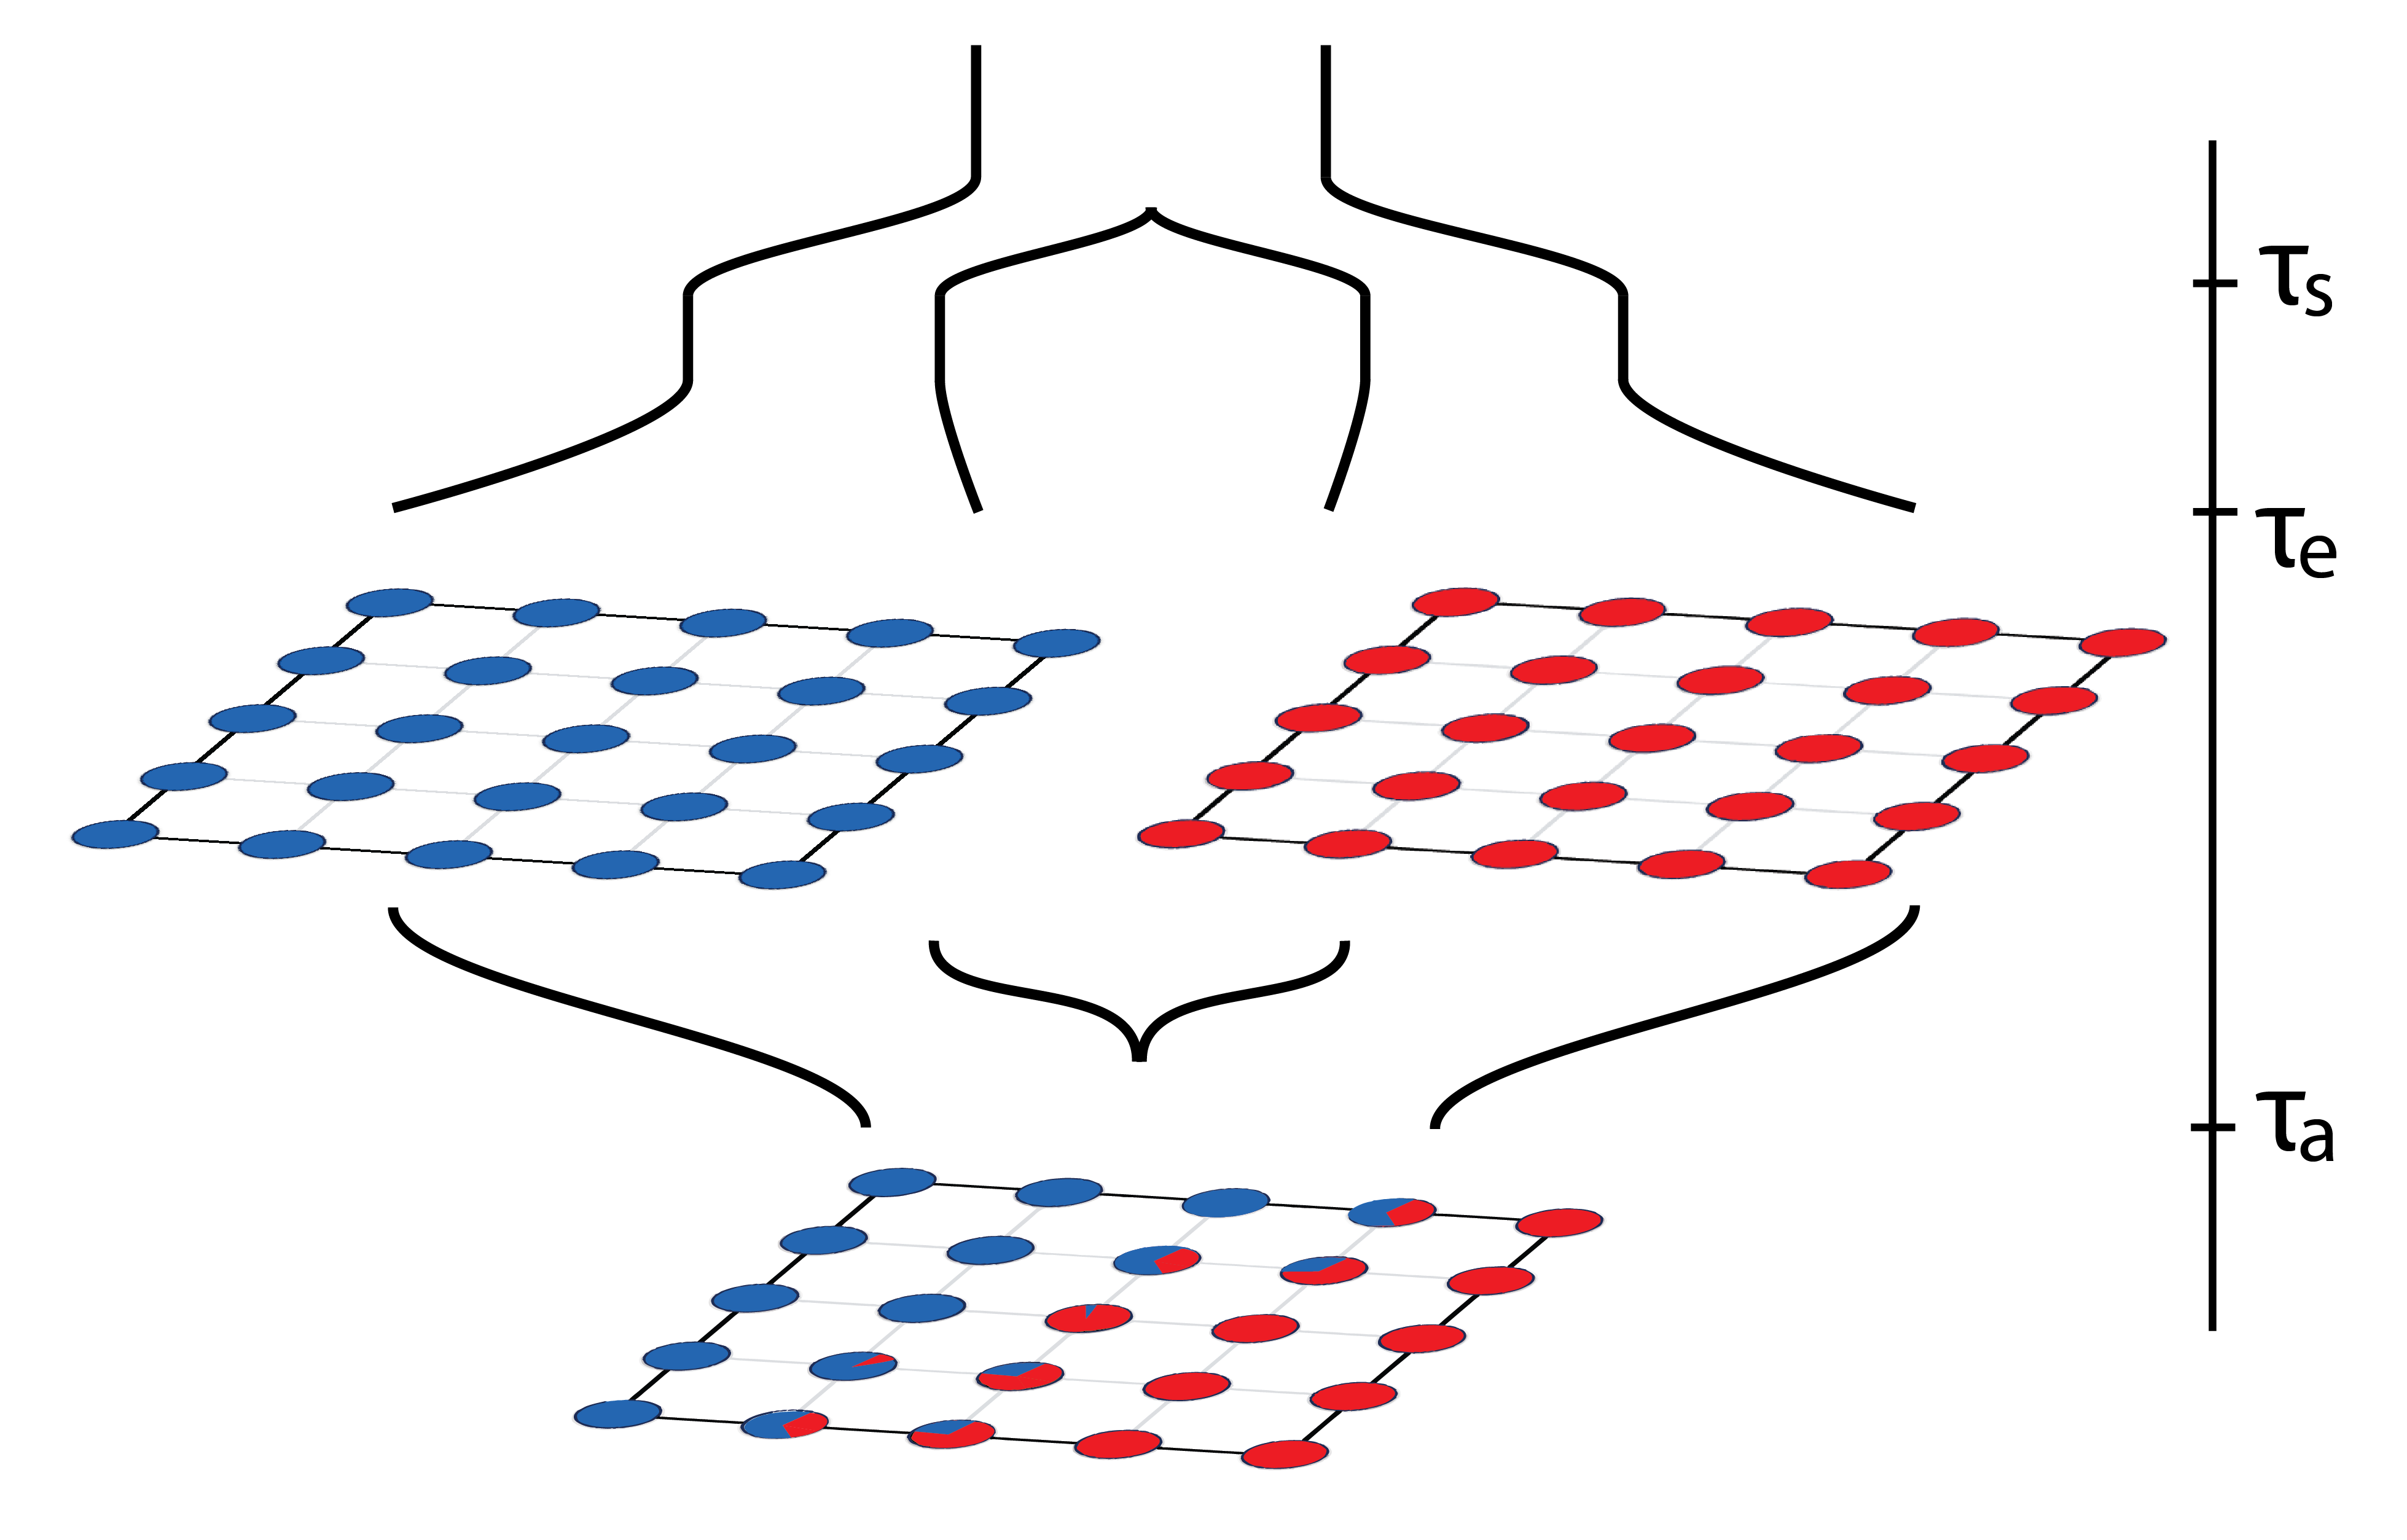
\includegraphics[width=4in,height=2.5in]{figs/sims/sim_setup.png}}
		\caption{Schematic of how we simulate datasets with continuous and discrete differentiation, using $K=2$ as an example.  
			    Going forward in time, the $K$ clusters split from a common ancestor at time $\tau_{\text{s}}$,
			    then each expand to colonize a lattice of demes with nearest-neighbor symmetric migration at time $\tau_{\text{e}}$,
			    then finally at time $\tau_{\text{a}}$ collapse into a single lattice consisting of demes 
			    with ancestry entirely in one or the other of the clusters,
			    or admixed between them.
			    }\label{sim_setup}
\end{figure}

\newpage
\begin{figure}
	\centering
		\subcaptionbox{$K=2$\label{simK1_nsp_pies:K2}}
			{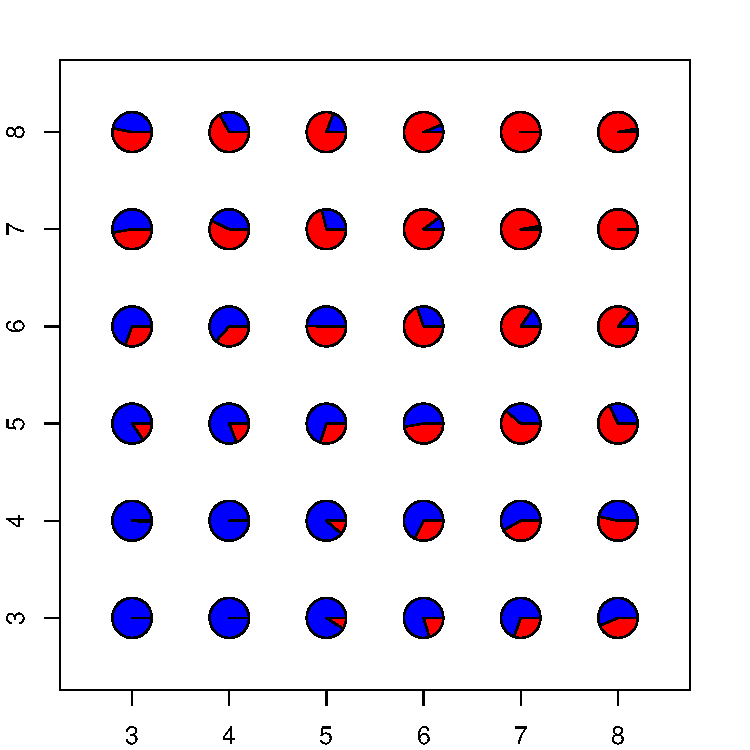
\includegraphics[width=1.8in,height=1.8in]{figs/sims/simK1_nsp_pies_K2.pdf}}
		\subcaptionbox{$K=3$\label{simK1_nsp_pies:K3}}
			{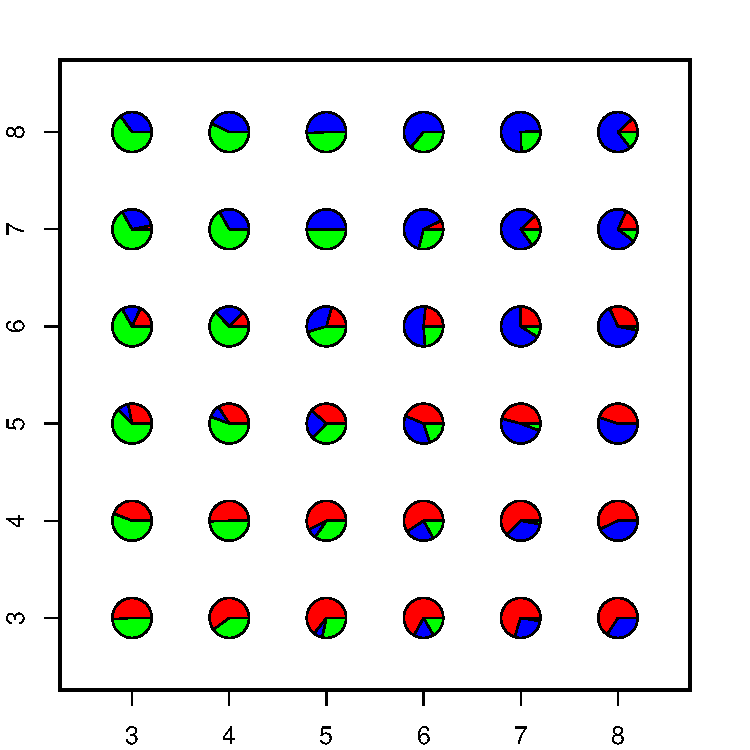
\includegraphics[width=1.8in,height=1.8in]{figs/sims/simK1_nsp_pies_K3.pdf}}
		\subcaptionbox{$K=4$\label{simK1_nsp_pies:K4}}
			{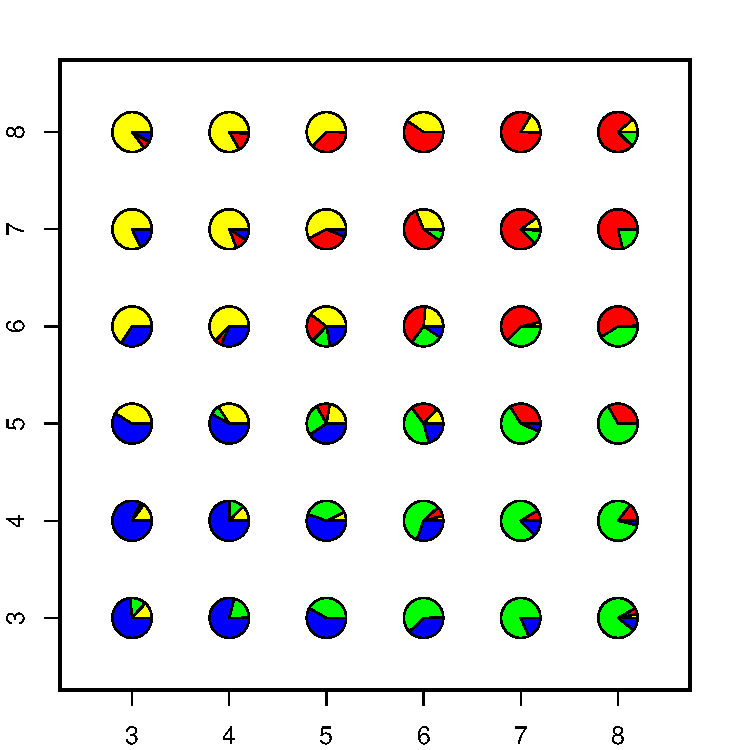
\includegraphics[width=1.8in,height=1.8in]{figs/sims/simK1_nsp_pies_K4.pdf}}
		\subcaptionbox{$K=5$\label{simK1_nsp_pies:K5}}
			{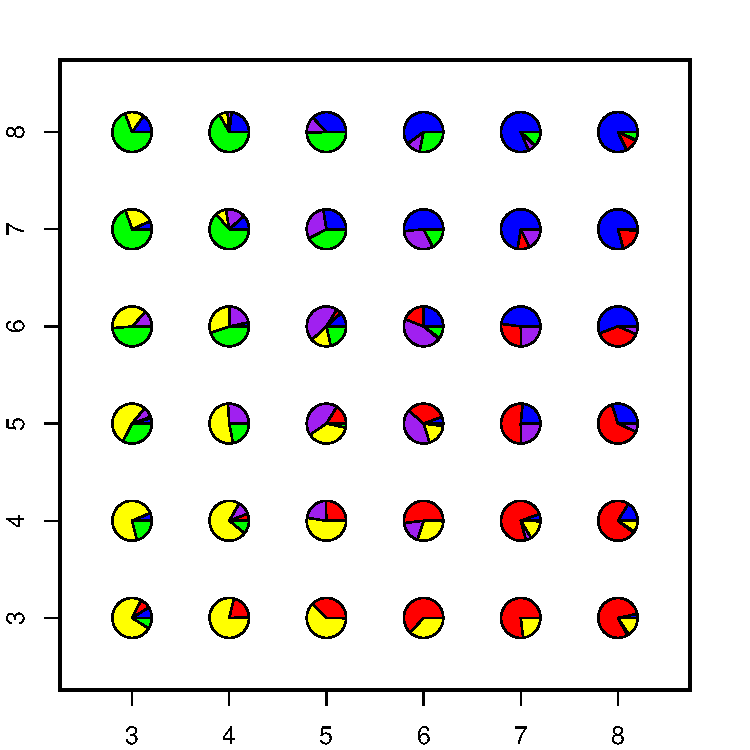
\includegraphics[width=1.8in,height=1.8in]{figs/sims/simK1_nsp_pies_K5.pdf}}
		\subcaptionbox{$K=6$\label{simK1_nsp_pies:K6}}
			{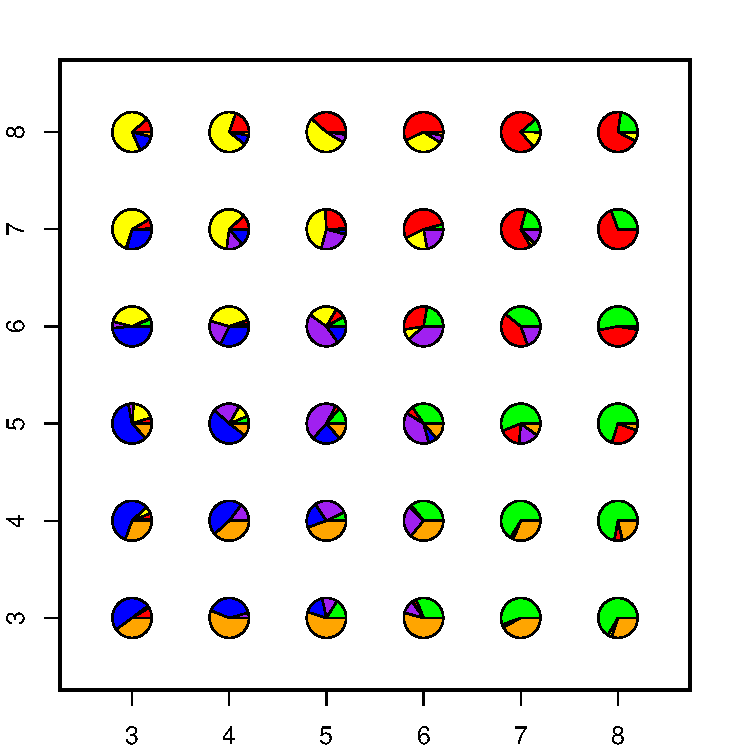
\includegraphics[width=1.8in,height=1.8in]{figs/sims/simK1_nsp_pies_K6.pdf}}
		\subcaptionbox{$K=7$\label{simK1_nsp_pies:K7}}
			{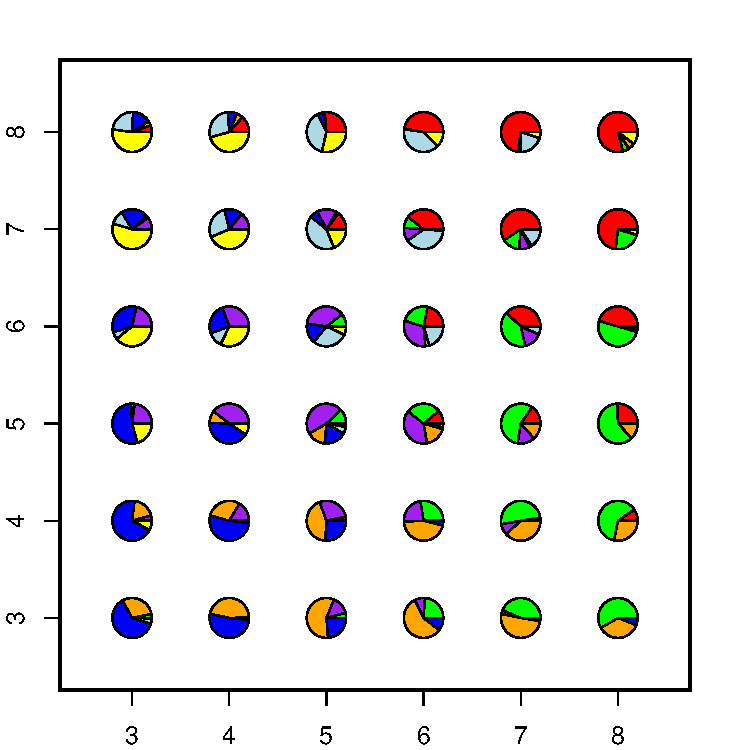
\includegraphics[width=1.8in,height=1.8in]{figs/sims/simK1_nsp_pies_K7.pdf}}
	\caption{
	Map of admixture proportions estimated using a nonspatial model for $K=2$ through 7.
	The data were simulated using a single cluster with nearest-neighbor symmetric migration between demes.
    }\label{simK1_nsp_pies}
\end{figure}

\begin{figure}
	\centering
		\subcaptionbox{$K=2$\label{simK1_sp_pies:K2}}
			{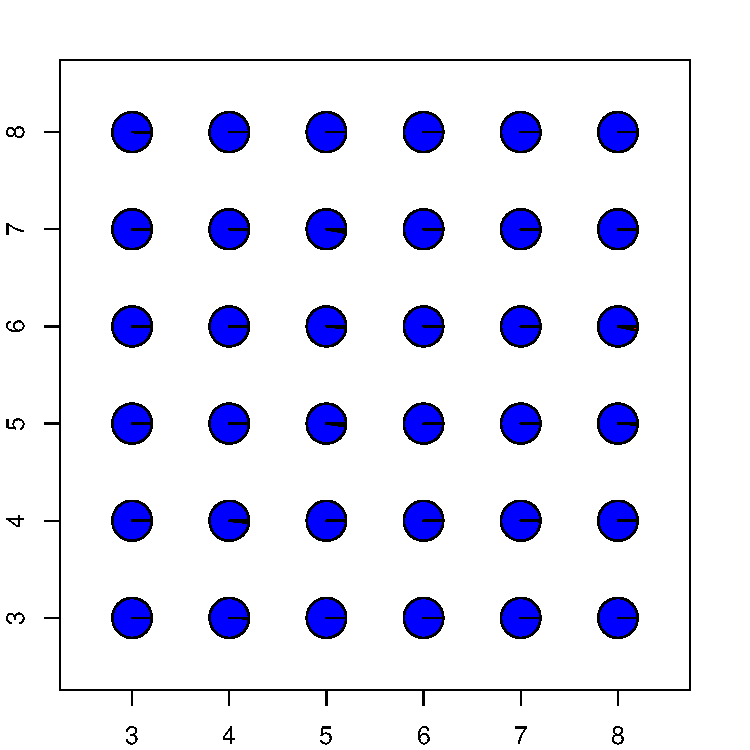
\includegraphics[width=1.8in,height=1.8in]{figs/sims/simK1_sp_pies_K2.pdf}}
		\subcaptionbox{$K=3$\label{simK1_sp_pies:K3}}
			{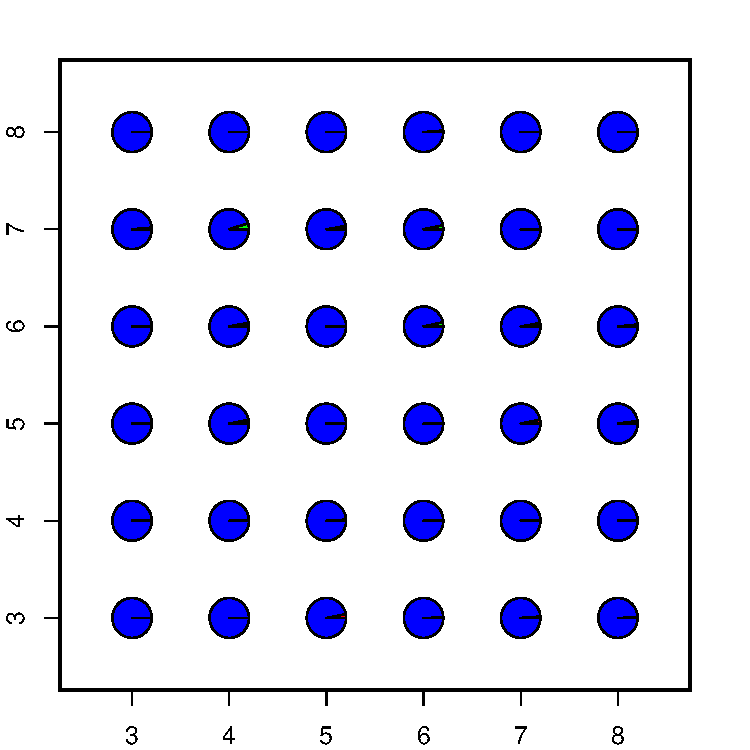
\includegraphics[width=1.8in,height=1.8in]{figs/sims/simK1_sp_pies_K3.pdf}}
		\subcaptionbox{$K=4$\label{simK1_sp_pies:K4}}
			{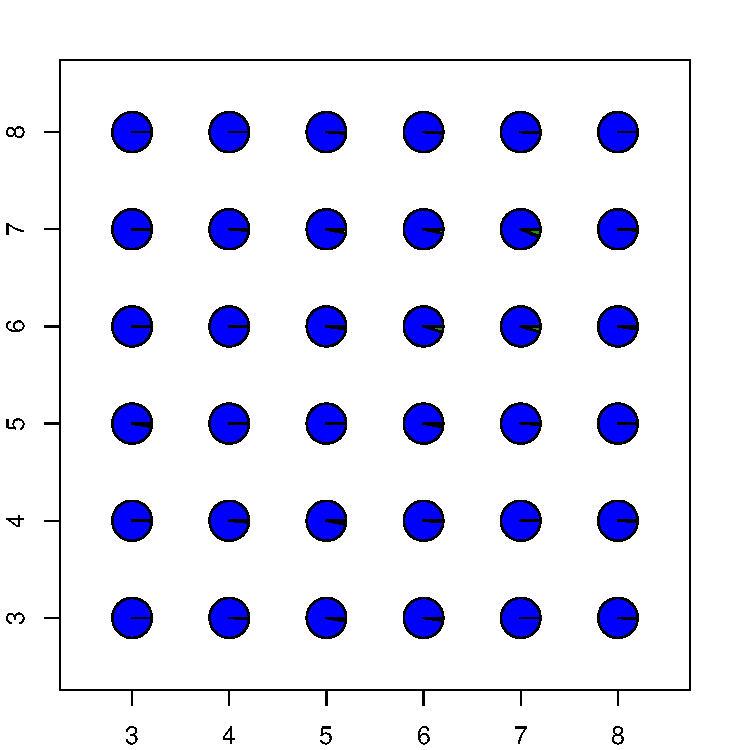
\includegraphics[width=1.8in,height=1.8in]{figs/sims/simK1_sp_pies_K4.pdf}}
		\subcaptionbox{$K=5$\label{simK1_sp_pies:K5}}
			{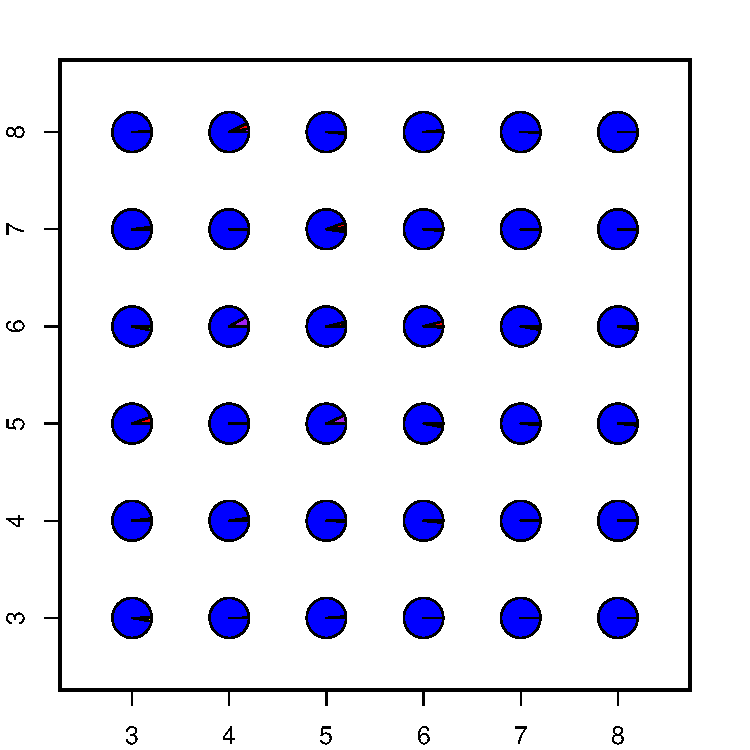
\includegraphics[width=1.8in,height=1.8in]{figs/sims/simK1_sp_pies_K5.pdf}}
		\subcaptionbox{$K=6$\label{simK1_sp_pies:K6}}
			{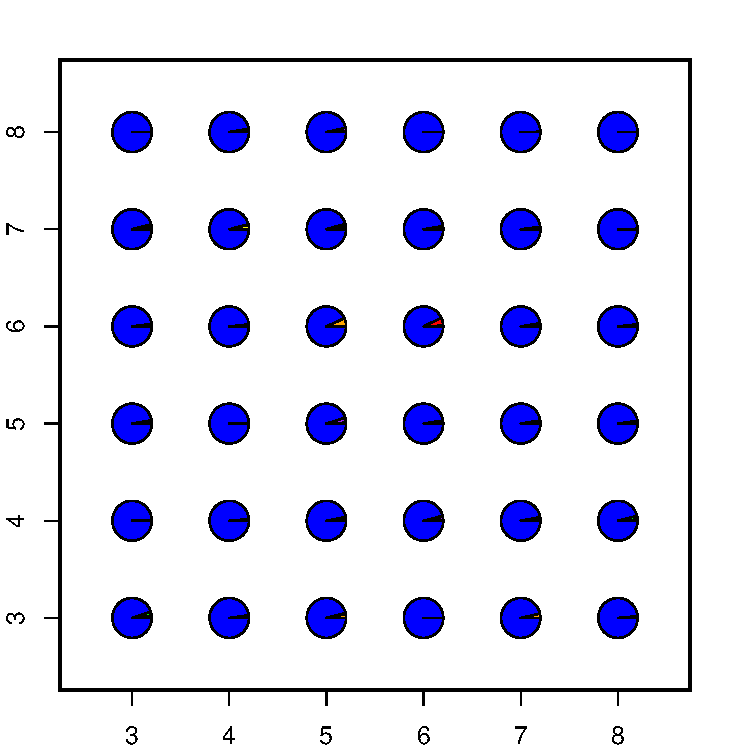
\includegraphics[width=1.8in,height=1.8in]{figs/sims/simK1_sp_pies_K6.pdf}}
		\subcaptionbox{$K=7$\label{simK1_sp_pies:K7}}
			{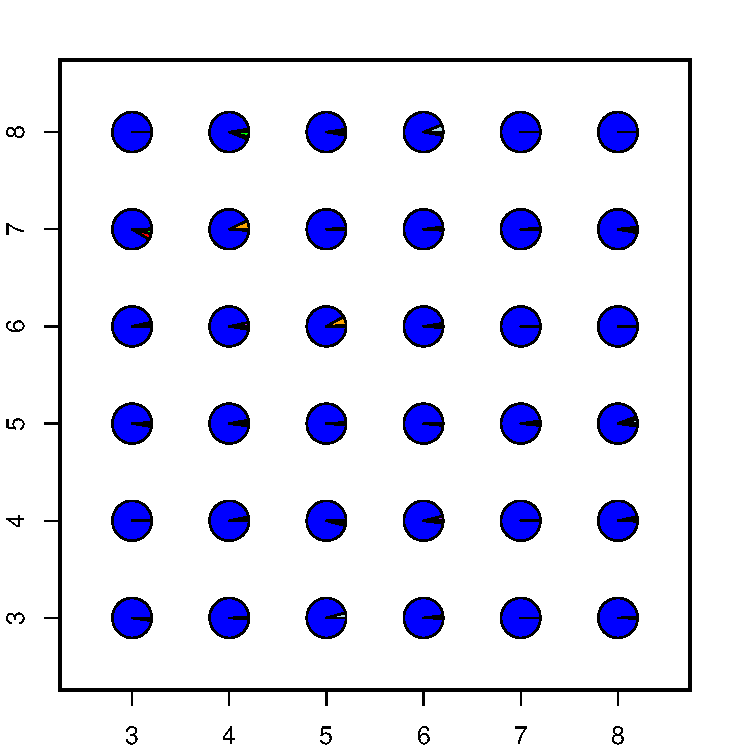
\includegraphics[width=1.8in,height=1.8in]{figs/sims/simK1_sp_pies_K7.pdf}}
	\caption{
	Map of admixture proportions estimated using a spatial model for $K=2$ through 7.
	The data were simulated using 1 cluster with nearest-neighbor symmetric migration between demes.
    }\label{simK1_sp_pies}
\end{figure}

\begin{figure}
	\centering
		{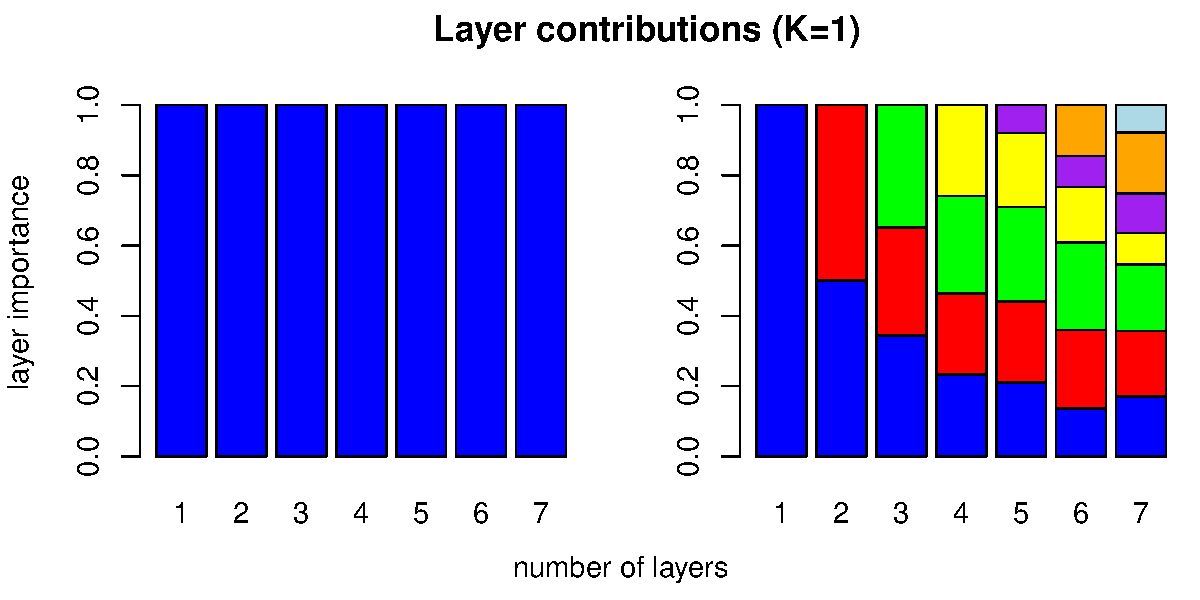
\includegraphics[width=5in,height=2.5in]{figs/sims/simK1_laycon_barplots.pdf}}
		\caption{
			Layer ``importance" (i.e., how much total covariance is contributed by each layer), 
			for all layers estimated in runs using $K = 1$ through 7 
			for the spatial model (left) and the nonspatial model (right).
			Data were simulated using $K=1$.
			For each value of $K$ along the x-axis, there are an equal number of layer contributions plotted.
		}\label{simK1_laycon}
\end{figure}

\begin{figure}
	\centering
		{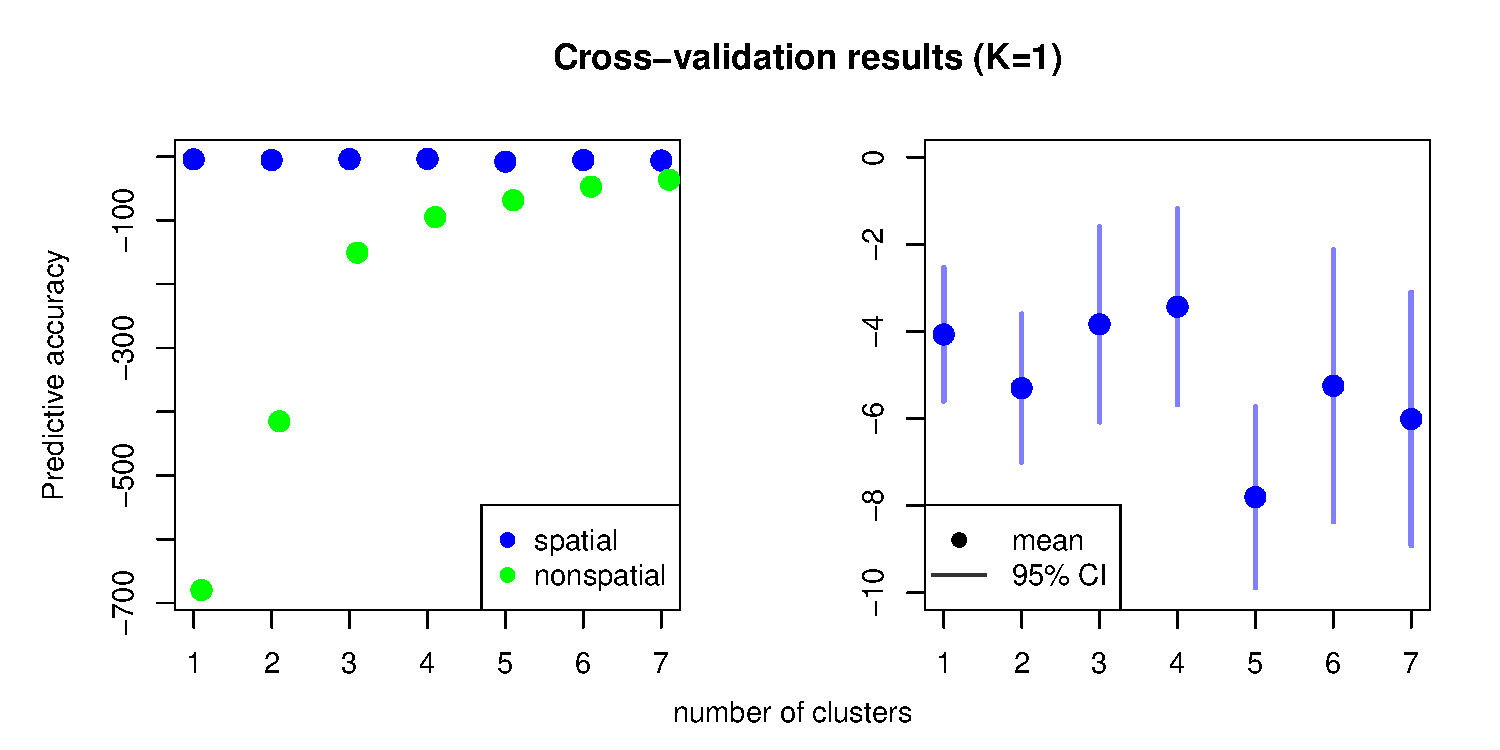
\includegraphics[width=5in,height=2.5in]{figs/sims/simK1_std_xval.pdf}}
		\caption{
			Cross-validation results for data simulated under $K=1$,
			comparing the spatial and nonspatial \texttt{conStruct} models run with $K=1$ through 7.  
			The right panel zooms in on just the spatial cross-validation results.
		}\label{simK1_xval}
\end{figure}


\newpage
\begin{figure}
	\centering
		\subcaptionbox{$K=2$\label{simK2_nsp_pies:K2}}
			{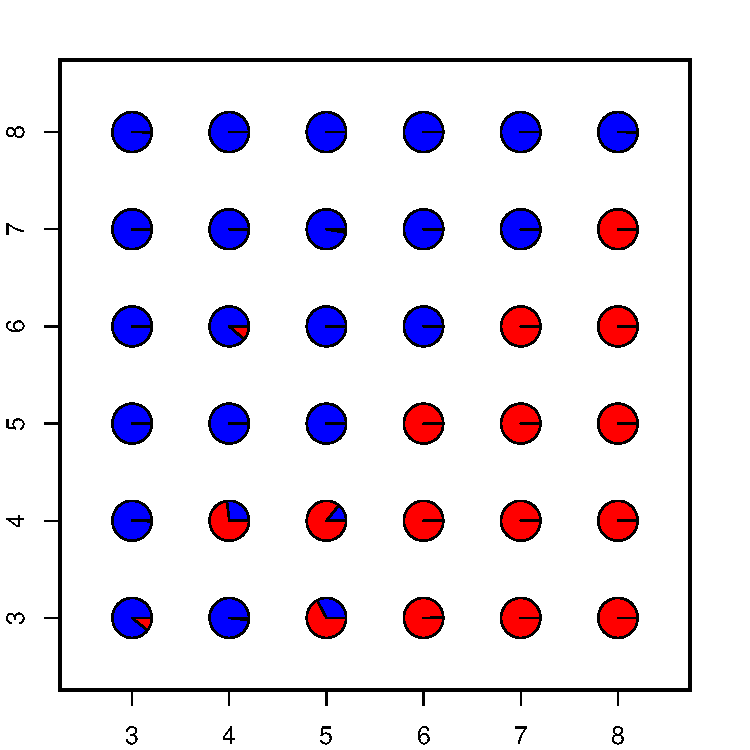
\includegraphics[width=1.8in,height=1.8in]{figs/sims/simK2_nsp_pies_K2.pdf}}
		\subcaptionbox{$K=3$\label{simK2_nsp_pies:K3}}
			{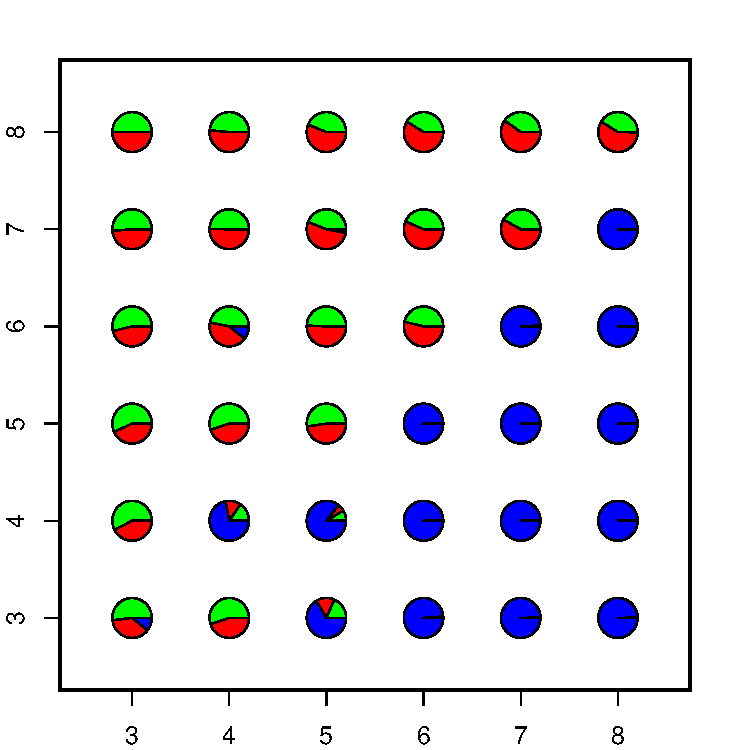
\includegraphics[width=1.8in,height=1.8in]{figs/sims/simK2_nsp_pies_K3.pdf}}
		\subcaptionbox{$K=4$\label{simK2_nsp_pies:K4}}
			{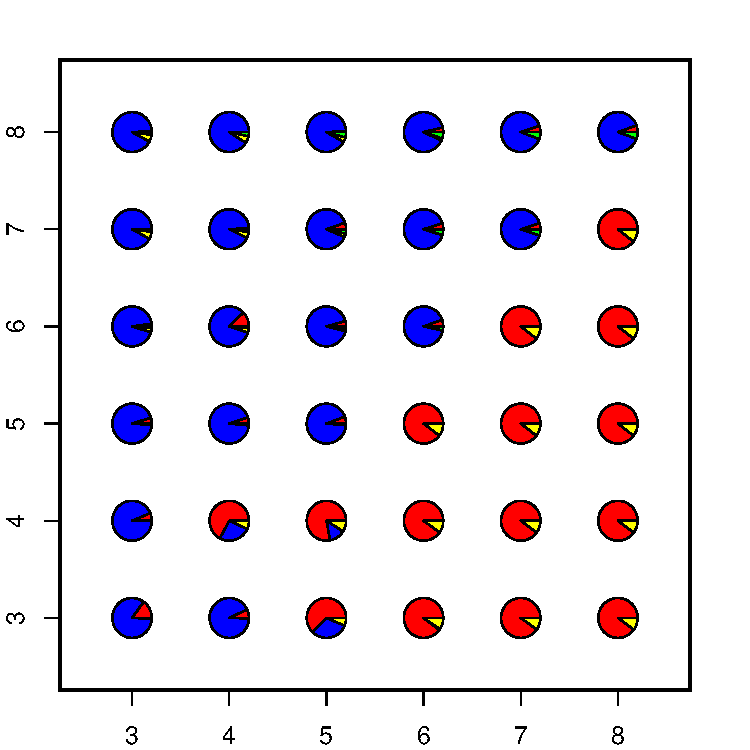
\includegraphics[width=1.8in,height=1.8in]{figs/sims/simK2_nsp_pies_K4.pdf}}
		\subcaptionbox{$K=5$\label{simK2_nsp_pies:K5}}
			{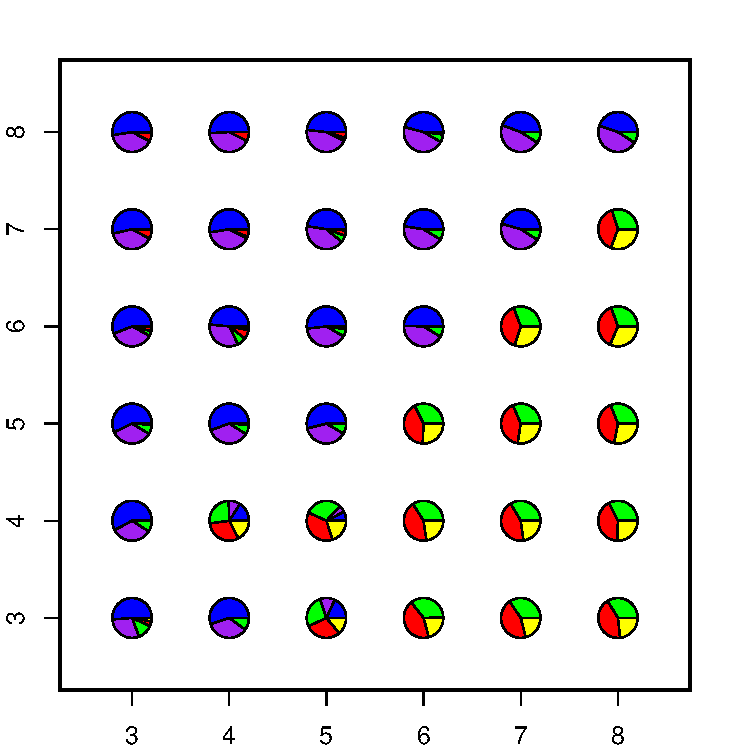
\includegraphics[width=1.8in,height=1.8in]{figs/sims/simK2_nsp_pies_K5.pdf}}
		\subcaptionbox{$K=6$\label{simK2_nsp_pies:K6}}
			{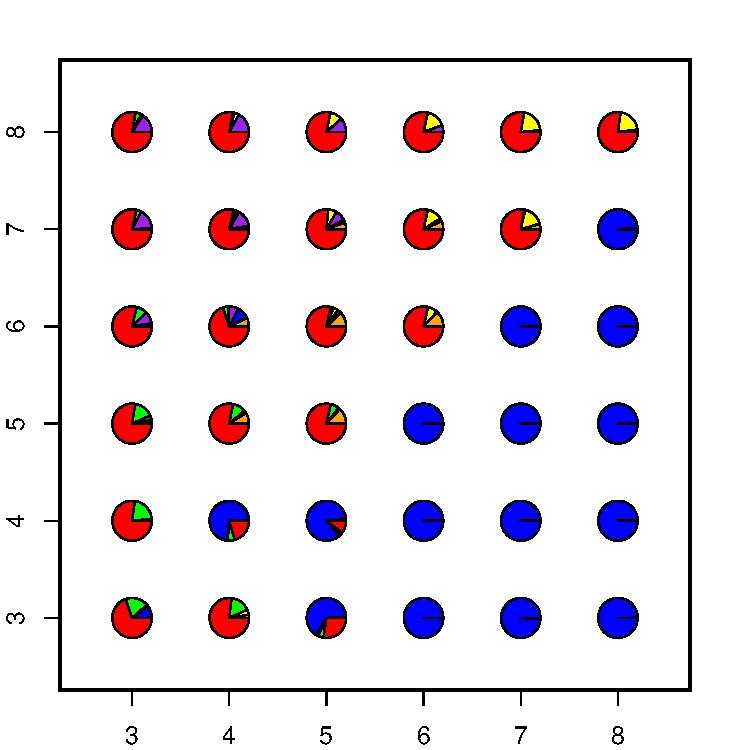
\includegraphics[width=1.8in,height=1.8in]{figs/sims/simK2_nsp_pies_K6.pdf}}
		\subcaptionbox{$K=7$\label{simK2_nsp_pies:K7}}
			{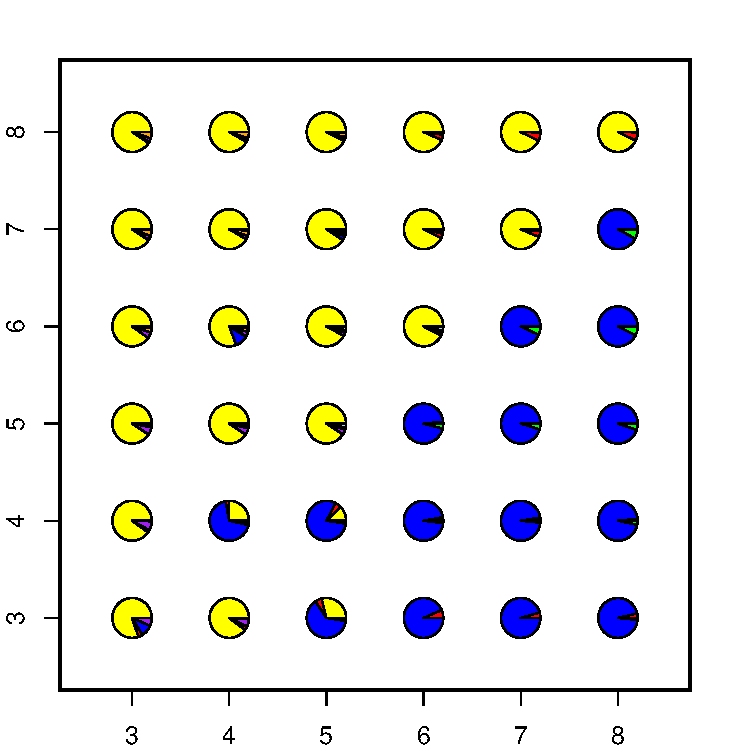
\includegraphics[width=1.8in,height=1.8in]{figs/sims/simK2_nsp_pies_K7.pdf}}
	\caption{
	Map of admixture proportions estimated using a nonspatial model for $K=2$ through 7.
	The data were simulated using two clusters with nearest-neighbor symmetric migration between demes.
    }\label{simK2_nsp_pies}
\end{figure}

\begin{figure}
	\centering
		\subcaptionbox{$K=2$\label{simK2_sp_pies:K2}}
			{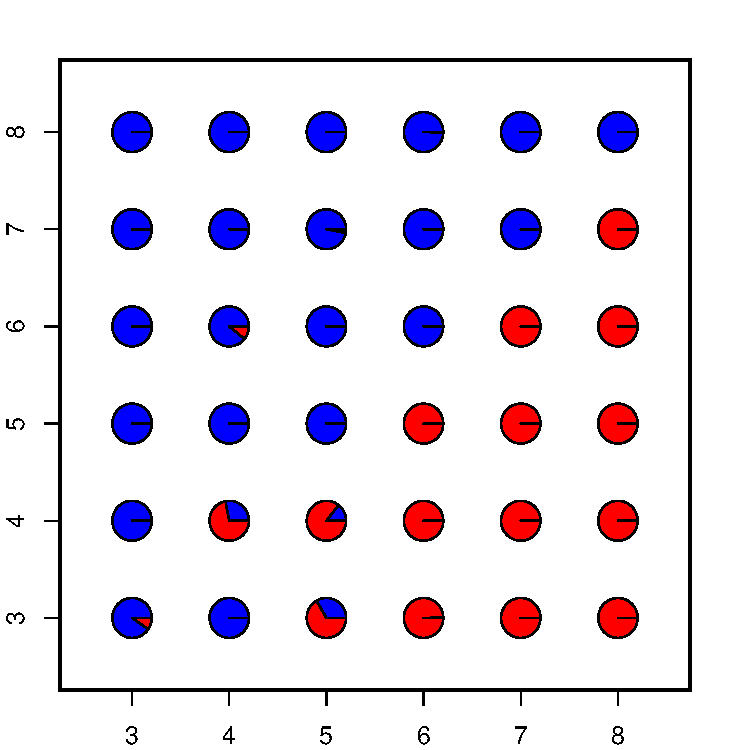
\includegraphics[width=1.8in,height=1.8in]{figs/sims/simK2_sp_pies_K2.pdf}}
		\subcaptionbox{$K=3$\label{simK2_sp_pies:K3}}
			{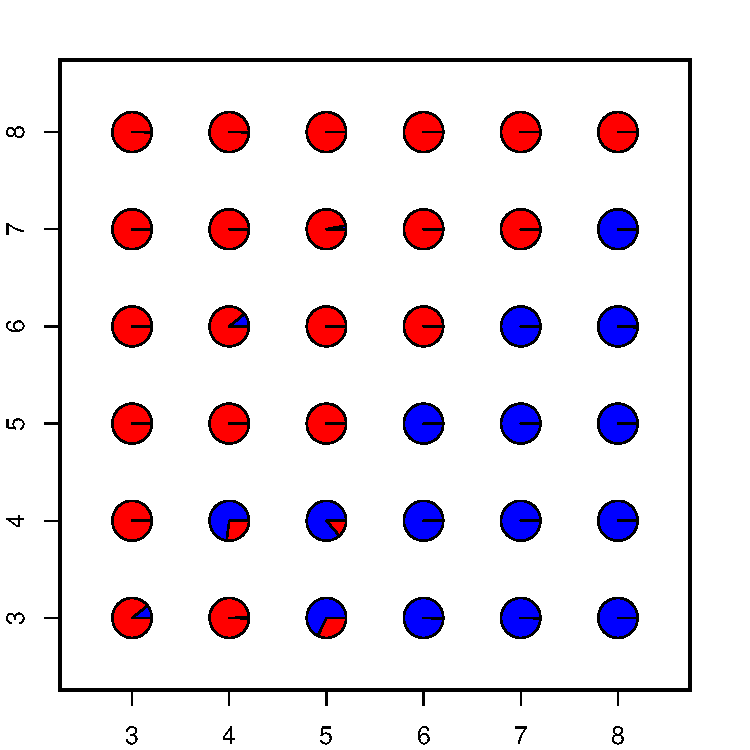
\includegraphics[width=1.8in,height=1.8in]{figs/sims/simK2_sp_pies_K3.pdf}}
		\subcaptionbox{$K=4$\label{simK2_sp_pies:K4}}
			{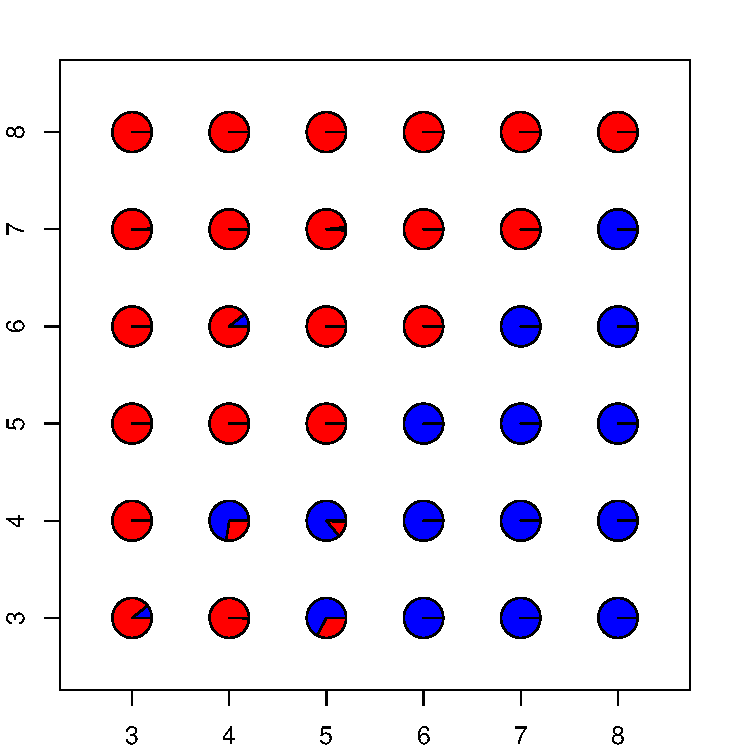
\includegraphics[width=1.8in,height=1.8in]{figs/sims/simK2_sp_pies_K4.pdf}}
		\subcaptionbox{$K=5$\label{simK2_sp_pies:K5}}
			{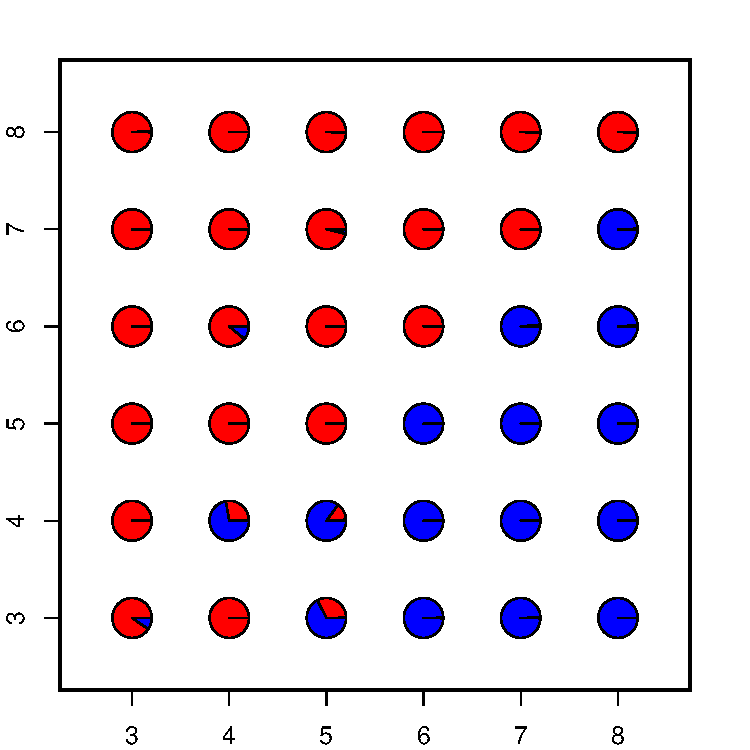
\includegraphics[width=1.8in,height=1.8in]{figs/sims/simK2_sp_pies_K5.pdf}}
		\subcaptionbox{$K=6$\label{simK2_sp_pies:K6}}
			{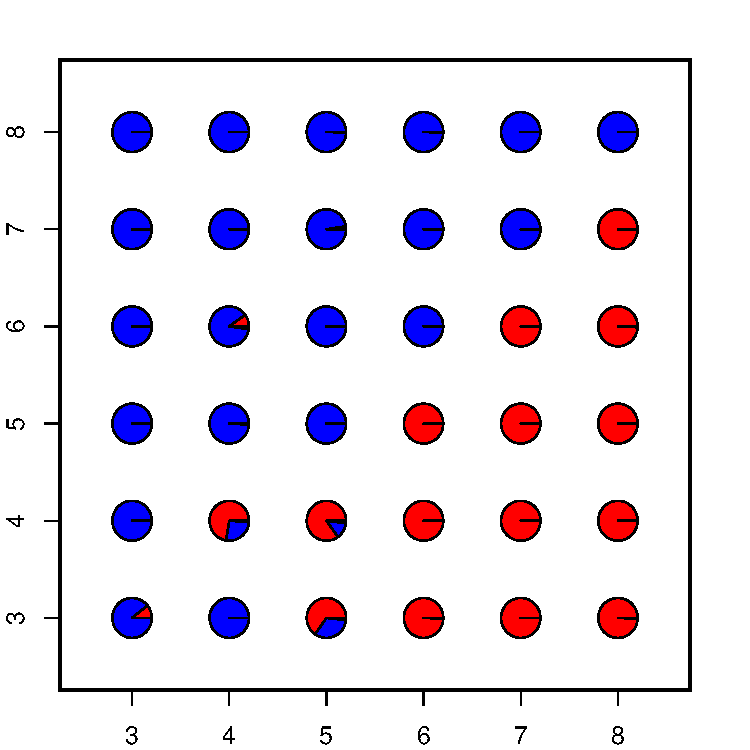
\includegraphics[width=1.8in,height=1.8in]{figs/sims/simK2_sp_pies_K6.pdf}}
		\subcaptionbox{$K=7$\label{simK2_sp_pies:K7}}
			{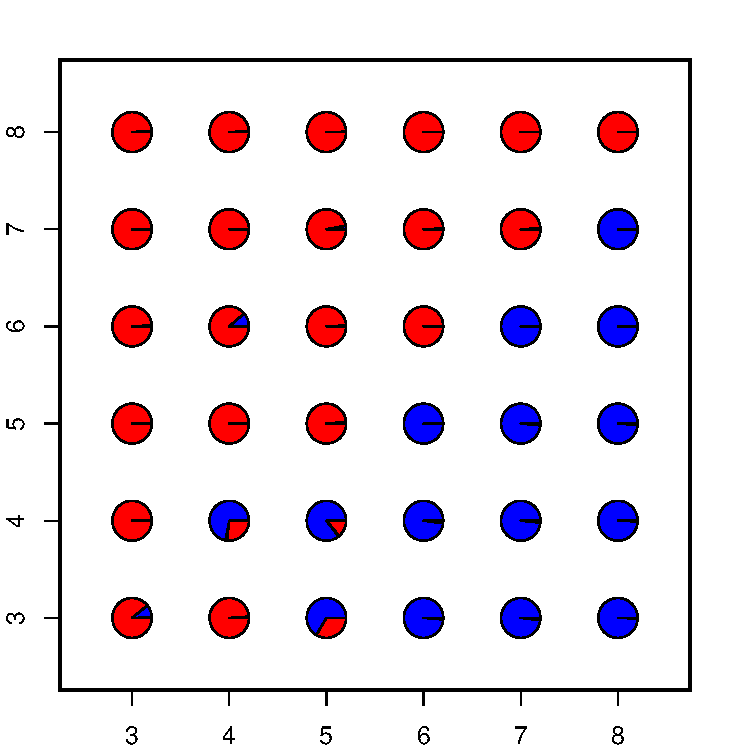
\includegraphics[width=1.8in,height=1.8in]{figs/sims/simK2_sp_pies_K7.pdf}}
	\caption{
	Map of admixture proportions estimated using a spatial model for $K=2$ through 7.
	The data were simulated using two clusters with nearest-neighbor symmetric migration between demes.
    }\label{simK2_sp_pies}
\end{figure}

\begin{figure}
	\centering
		{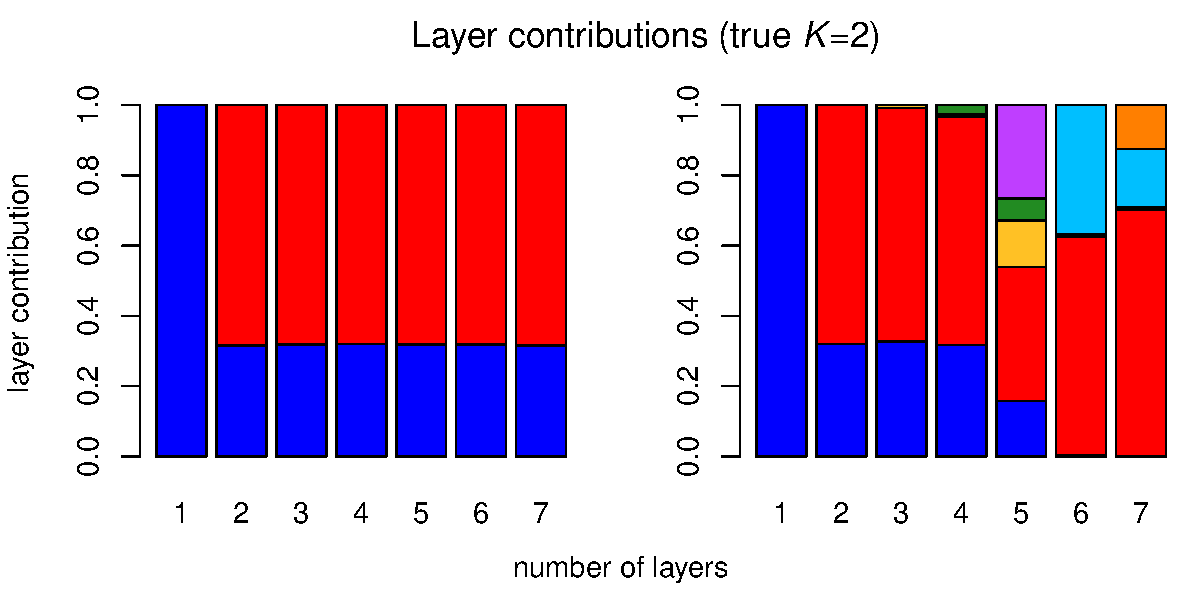
\includegraphics[width=5in,height=2.5in]{figs/sims/simK2_laycon_barplots.pdf}}
		\caption{
			Layer ``importance" (i.e., how much total covariance is contributed by each layer), 
			for all layers estimated in runs using $K = 1$ through 7 
			for the spatial model (left) and the nonspatial model (right).
			Data were simulated using $K=2$.
			For each value of $K$ along the x-axis, there are an equal number of layer contributions plotted.
		}\label{simK2_laycon}
\end{figure}

\begin{figure}
	\centering
		{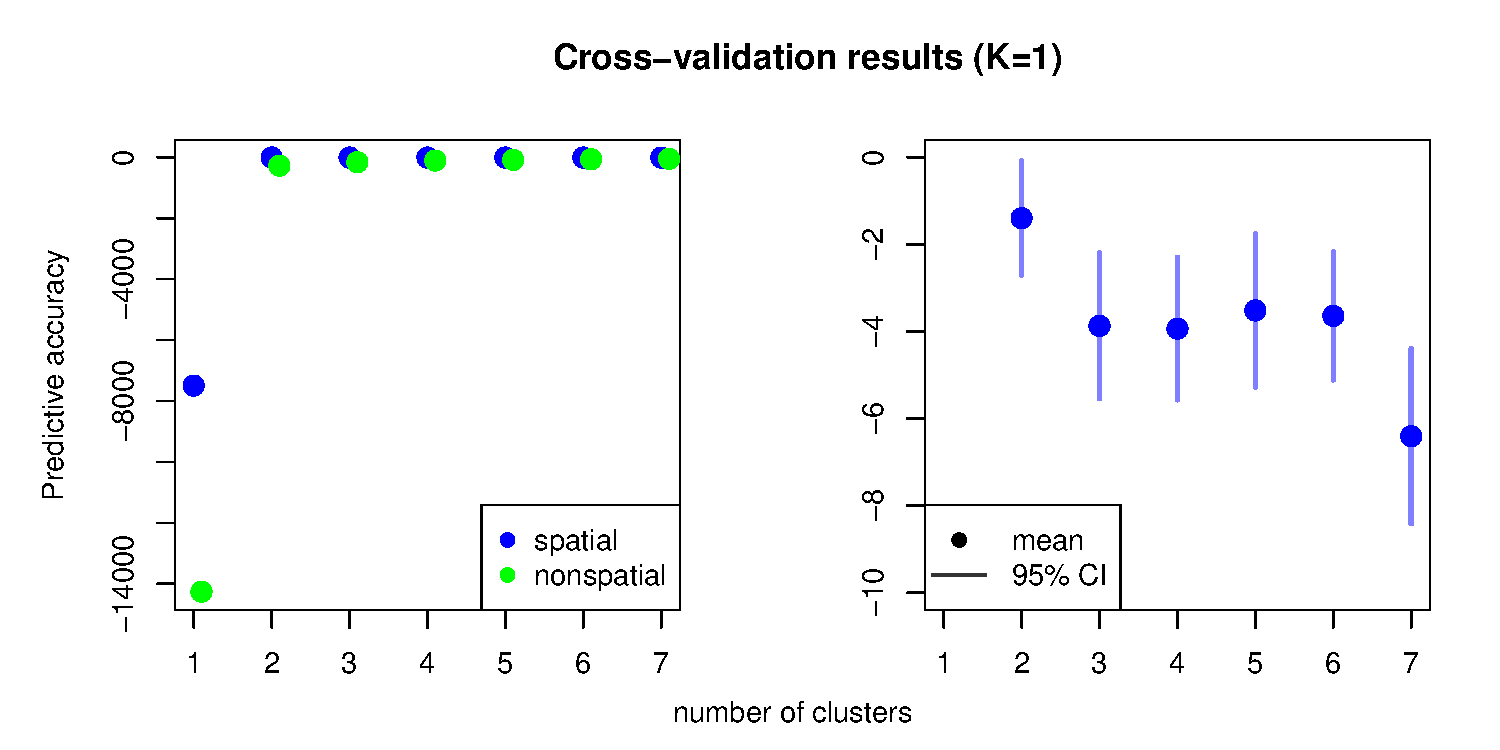
\includegraphics[width=5in,height=2.5in]{figs/sims/simK2_std_xval.pdf}}
		\caption{
			Cross-validation results for data simulated under $K=2$,
			comparing the spatial and nonspatial \texttt{conStruct} models run with $K=1$ through 7.  
			The right panel zooms in on just the spatial cross-validation results.
		}\label{simK2_xval}
\end{figure}

\begin{figure}
	\centering
		{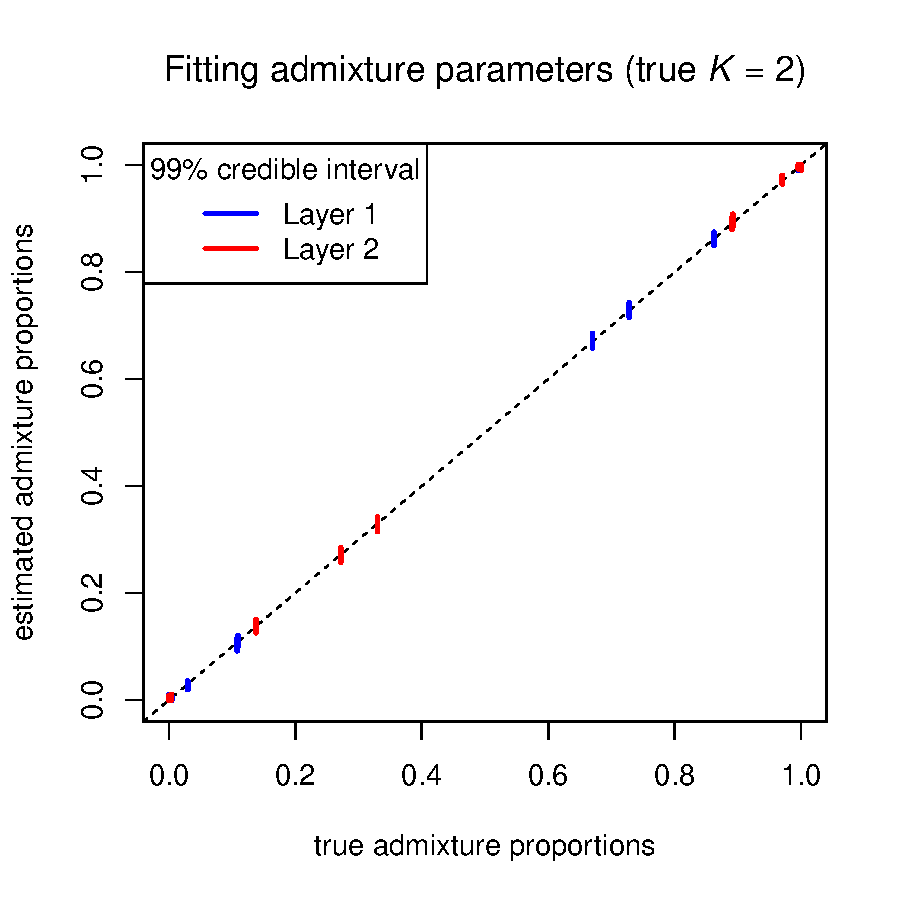
\includegraphics[width=4in,height=4in]{figs/sims/simK2_adprop_fit.pdf}}
		\caption{
			Plot of \texttt{conStruct} ability to correctly estimate admixture proportions on simulated data.
			Results are from an analysis with a spatial model using $K=2$.
		}\label{simK2_adprop_fit}
\end{figure}

\begin{figure}
	\centering
		\subcaptionbox{$K=2$\label{simK3_nsp_pies:K2}}
			{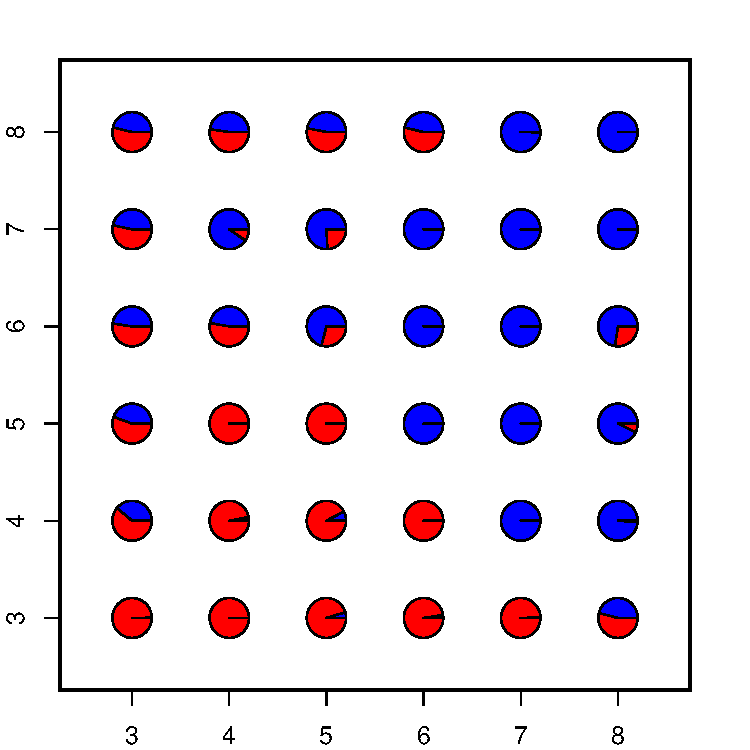
\includegraphics[width=1.8in,height=1.8in]{figs/sims/simK3_nsp_pies_K2.pdf}}
		\subcaptionbox{$K=3$\label{simK3_nsp_pies:K3}}
			{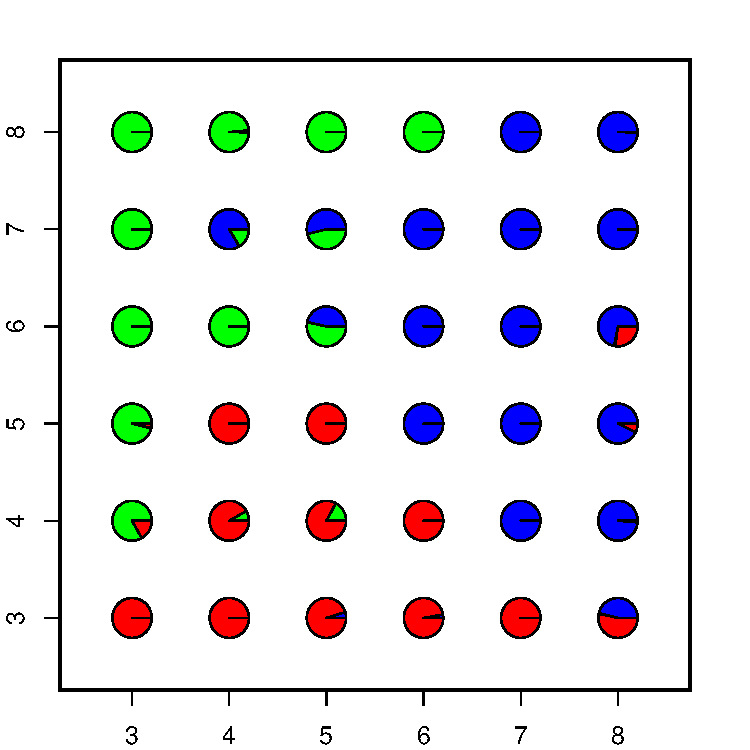
\includegraphics[width=1.8in,height=1.8in]{figs/sims/simK3_nsp_pies_K3.pdf}}
		\subcaptionbox{$K=4$\label{simK3_nsp_pies:K4}}
			{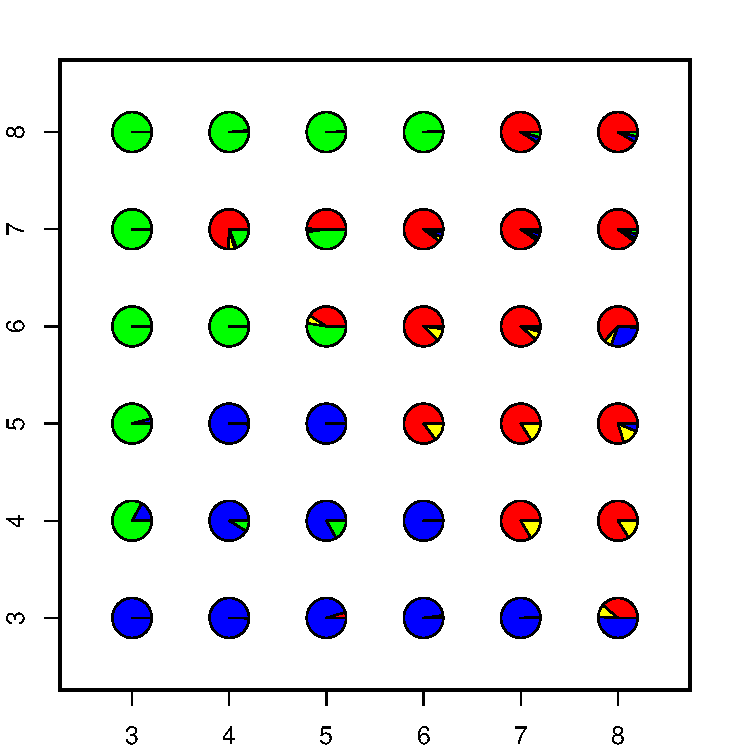
\includegraphics[width=1.8in,height=1.8in]{figs/sims/simK3_nsp_pies_K4.pdf}}
		\subcaptionbox{$K=5$\label{simK3_nsp_pies:K5}}
			{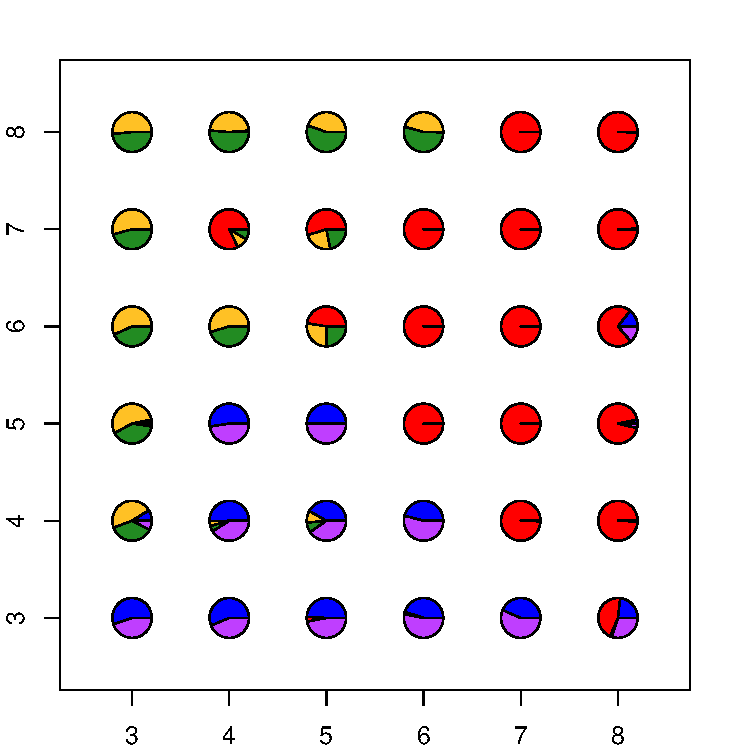
\includegraphics[width=1.8in,height=1.8in]{figs/sims/simK3_nsp_pies_K5.pdf}}
		\subcaptionbox{$K=6$\label{simK3_nsp_pies:K6}}
			{\includegraphics[width=1.8in,height=1.8in]{figs/sims/simK3_nsp_pies_K6.pdf}}
		\subcaptionbox{$K=7$\label{simK3_nsp_pies:K7}}
			{\includegraphics[width=1.8in,height=1.8in]{figs/sims/simK3_nsp_pies_K7.pdf}}
	\caption{
	Map of admixture proportions estimated using a nonspatial model for $K=2$ through 7.
	The data were simulated using three clusters with nearest-neighbor symmetric migration between demes.
    }\label{simK3_nsp_pies}
\end{figure}

\begin{figure}
	\centering
		\subcaptionbox{$K=2$\label{simK3_sp_pies:K2}}
			{\includegraphics[width=1.8in,height=1.8in]{figs/sims/simK3_sp_pies_K2.pdf}}
		\subcaptionbox{$K=3$\label{simK3_sp_pies:K3}}
			{\includegraphics[width=1.8in,height=1.8in]{figs/sims/simK3_sp_pies_K3.pdf}}
		\subcaptionbox{$K=4$\label{simK3_sp_pies:K4}}
			{\includegraphics[width=1.8in,height=1.8in]{figs/sims/simK3_sp_pies_K4.pdf}}
		\subcaptionbox{$K=5$\label{simK3_sp_pies:K5}}
			{\includegraphics[width=1.8in,height=1.8in]{figs/sims/simK3_sp_pies_K5.pdf}}
		\subcaptionbox{$K=6$\label{simK3_sp_pies:K6}}
			{\includegraphics[width=1.8in,height=1.8in]{figs/sims/simK3_sp_pies_K6.pdf}}
		\subcaptionbox{$K=7$\label{simK3_sp_pies:K7}}
			{\includegraphics[width=1.8in,height=1.8in]{figs/sims/simK3_sp_pies_K7.pdf}}
	\caption{
	Map of admixture proportions estimated using a spatial model for $K=2$ through 7.
	The data were simulated using three clusters with nearest-neighbor symmetric migration between demes.
    }\label{simK3_sp_pies}
\end{figure}
\clearpage

\begin{figure}
	\centering
		{\includegraphics[width=5in,height=2.5in]{figs/sims/simK3_laycon_barplots.pdf}}
		\caption{
			Layer ``importance" (i.e., how much total covariance is contributed by each layer), 
			for all layers estimated in runs using $K = 1$ through 7 
			for the spatial model (left) and the nonspatial model (right).
			Data were simulated using $K=3$.
			For each value of $K$ along the x-axis, there are an equal number of layer contributions plotted.
		}\label{simK3_laycon}
\end{figure}

\begin{figure}
	\centering
		{\includegraphics[width=5in,height=2.5in]{figs/sims/simK3_std_xval.pdf}}
		\caption{
			Cross-validation results for data simulated under $K=3$,
			comparing the spatial and nonspatial \texttt{conStruct} models run with $K=1$ through 7.  
			The right panel zooms in on just the spatial cross-validation results.
		}\label{simK3_xval}
\end{figure}

\begin{figure}
	\centering
		{\includegraphics[width=4in,height=4in]{figs/sims/simK3_adprop_fit.pdf}}
		\caption{
			Plot of \texttt{conStruct} ability to correctly estimate admixture proportions on simulated data.
			Results are from an analysis with a spatial model using $K=3$.
		}\label{simK3_adprop_fit}
\end{figure}

\begin{figure}
	\centering
		{\includegraphics[width=6in,height=2.25in]{figs/fastStr/fastStr_simK1_pies.pdf}}
	\caption{
	Map of admixture proportions estimated using fastSTRUCTURE \citep{fastStructure} for $K=2$ through 4.
	The data were simulated using one cluster with nearest-neighbor symmetric migration between demes.
    }\label{fastStr_simK1}
\end{figure}

\begin{figure}
	\centering
		{\includegraphics[width=6in,height=2.25in]{figs/fastStr/fastStr_simK2_pies.pdf}}
	\caption{
	Map of admixture proportions estimated using fastSTRUCTURE \citep{fastStructure} for $K=2$ through 4.
	The data were simulated using two clusters with nearest-neighbor symmetric migration between demes.
    }\label{fastStr_simK2}
\end{figure}

\begin{figure}
	\centering
		{\includegraphics[width=6in,height=2.25in]{figs/fastStr/fastStr_simK3_pies.pdf}}
	\caption{
	Map of admixture proportions estimated using fastSTRUCTURE \citep{fastStructure} for $K=2$ through 4.
	The data were simulated using three clusters with nearest-neighbor symmetric migration between demes.
    }\label{fastStr_simK3}
\end{figure}

\begin{figure}
	\centering
		{\includegraphics[width=6in,height=5in]{figs/populus/populus_sampling_map.pdf}}
	\caption{
	Map of the sampled \textit{Populus} populations included in the analysis.
	The color of the sampling location denotes the putative species.
    }\label{populus_map}
\end{figure}

\begin{figure}
	\centering
		\subcaptionbox{$K=2$\label{populus_sp_pies:K2}}
			{\includegraphics[width=1.8in,height=1.8in]{figs/populus/populus_sp2.pdf}}
		\subcaptionbox{$K=3$\label{populus_sp_pies:K3}}
			{\includegraphics[width=1.8in,height=1.8in]{figs/populus/populus_sp3.pdf}}
		\subcaptionbox{$K=4$\label{populus_sp_pies:K4}}
			{\includegraphics[width=1.8in,height=1.8in]{figs/populus/populus_sp4.pdf}}
		\subcaptionbox{$K=5$\label{populus_sp_pies:K5}}
			{\includegraphics[width=1.8in,height=1.8in]{figs/populus/populus_sp5.pdf}}
		\subcaptionbox{$K=6$\label{populus_sp_pies:K6}}
			{\includegraphics[width=1.8in,height=1.8in]{figs/populus/populus_sp6.pdf}}
		\subcaptionbox{$K=7$\label{populus_sp_pies:K7}}
			{\includegraphics[width=1.8in,height=1.8in]{figs/populus/populus_sp7.pdf}}
	\caption{
	Map of admixture proportions estimated for the \textit{Populus} dataset 
	using the spatial model for $K=2$ through 7.
    }\label{populus_sp_pies}
\end{figure}

\begin{figure}
	\centering
		\subcaptionbox{$K=2$\label{populus_nsp_pies:K2}}
			{\includegraphics[width=1.8in,height=1.8in]{figs/populus/populus_nsp2.pdf}}
		\subcaptionbox{$K=3$\label{populus_nsp_pies:K3}}
			{\includegraphics[width=1.8in,height=1.8in]{figs/populus/populus_nsp3.pdf}}
		\subcaptionbox{$K=4$\label{populus_nsp_pies:K4}}
			{\includegraphics[width=1.8in,height=1.8in]{figs/populus/populus_nsp4.pdf}}
		\subcaptionbox{$K=5$\label{populus_nsp_pies:K5}}
			{\includegraphics[width=1.8in,height=1.8in]{figs/populus/populus_nsp5.pdf}}
		\subcaptionbox{$K=6$\label{populus_nsp_pies:K6}}
			{\includegraphics[width=1.8in,height=1.8in]{figs/populus/populus_nsp6.pdf}}
		\subcaptionbox{$K=7$\label{populus_nsp_pies:K7}}
			{\includegraphics[width=1.8in,height=1.8in]{figs/populus/populus_nsp7.pdf}}
	\caption{
	Map of admixture proportions estimated for the \textit{Populus} dataset 
	using the nonspatial model for $K=2$ through 7.
    }\label{populus_nsp_pies}
\end{figure}

\begin{figure}
	\centering
		{\includegraphics[width=6in,height=4in]{figs/populus/populus_sp_clst_covs.pdf}}
	\caption{
	Plots showing the cluster-specific parametric covariance IBD-curves 
	estimated for the \textit{Populus} data using 
	the spatial \texttt{conStruct} model run with $K=1$ through 6.
	Line colors are consistent with cluster colors in Fig \ref{populus_sp_pies}.
	Points are colored by the species they are a covariance between:
	black on black points are sample covariances between populations of \textit{Populus balsamifera};
	green on black points are sample covariances between \bals{} and \tri{};
	green on green points are sample covariances between \tri{} and \tri{}.
    }\label{populus_sp_clst_covs}
\end{figure}

\begin{figure}
	\centering
		{\includegraphics[width=6in,height=4in]{figs/populus/populus_nsp_clst_covs.pdf}}
	\caption{
	Plots showing the cluster-specific parametric covariances 
	estimated for the \textit{Populus} data using 
	the nonspatial \texttt{conStruct} model run with $K=1$ through 6.
	Line colors are consistent with cluster colors in Fig \ref{populus_nsp_pies}.
	Points are colored by the species they are a covariance between:
	black on black points are sample covariances between populations of \textit{Populus balsamifera};
	green on black points are sample covariances between \bals{} and \tri{};
	green on green points are sample covariances between \tri{} and \tri{}.
    }\label{populus_nsp_clst_covs}
\end{figure}

\begin{figure}
	\centering
		{\includegraphics[width=6in,height=3in]{figs/populus/populus_laycon_barplots.pdf}}
	\caption{
	Layer ``contributions" (i.e., how much total covariance is contributed by each layer), 
	for all layers estimated in runs using $K = 1$ through 7 
	for the spatial model (left) and the nonspatial model (right).
	For each value of $K$ along the x-axis, there are an equal number of layer contributions plotted.
	Colors are consistent with Figs \ref{populus_sp_pies}, \ref{populus_sp_clst_covs}, \ref{populus_nsp_pies}, and \ref{populus_nsp_clst_covs}.
    }\label{populus_laycon}
\end{figure}

\begin{figure}
	\centering
		\subcaptionbox{$K=2$\label{bear_sp_pies:K2}}
			{\includegraphics[width=1.8in,height=1.8in]{figs/bears/bear_sp2.pdf}}
		\subcaptionbox{$K=3$\label{bear_sp_pies:K3}}
			{\includegraphics[width=1.8in,height=1.8in]{figs/bears/bear_sp3.pdf}}
		\subcaptionbox{$K=4$\label{bear_sp_pies:K4}}
			{\includegraphics[width=1.8in,height=1.8in]{figs/bears/bear_sp4.pdf}}
		\subcaptionbox{$K=5$\label{bear_sp_pies:K5}}
			{\includegraphics[width=1.8in,height=1.8in]{figs/bears/bear_sp5.pdf}}
		\subcaptionbox{$K=6$\label{bear_sp_pies:K6}}
			{\includegraphics[width=1.8in,height=1.8in]{figs/bears/bear_sp6.pdf}}
		\subcaptionbox{$K=7$\label{bear_sp_pies:K7}}
			{\includegraphics[width=1.8in,height=1.8in]{figs/bears/bear_sp7.pdf}}
	\caption{
	Map of admixture proportions estimated for the \textit{bear} dataset 
	using the spatial model for $K=2$ through 7.
    }\label{bear_sp_pies}
\end{figure}

\begin{figure}
	\centering
		\subcaptionbox{$K=2$\label{bear_nsp_pies:K2}}
			{\includegraphics[width=1.8in,height=1.8in]{figs/bears/bear_nsp2.pdf}}
		\subcaptionbox{$K=3$\label{bear_nsp_pies:K3}}
			{\includegraphics[width=1.8in,height=1.8in]{figs/bears/bear_nsp3.pdf}}
		\subcaptionbox{$K=4$\label{bear_nsp_pies:K4}}
			{\includegraphics[width=1.8in,height=1.8in]{figs/bears/bear_nsp4.pdf}}
		\subcaptionbox{$K=5$\label{bear_nsp_pies:K5}}
			{\includegraphics[width=1.8in,height=1.8in]{figs/bears/bear_nsp5.pdf}}
		\subcaptionbox{$K=6$\label{bear_nsp_pies:K6}}
			{\includegraphics[width=1.8in,height=1.8in]{figs/bears/bear_nsp6.pdf}}
		\subcaptionbox{$K=7$\label{bear_nsp_pies:K7}}
			{\includegraphics[width=1.8in,height=1.8in]{figs/bears/bear_nsp7.pdf}}
	\caption{
	Map of admixture proportions estimated for the \textit{bear} dataset 
	using the nonspatial model for $K=2$ through 7.
    }\label{bear_nsp_pies}
\end{figure}

\begin{figure}
	\centering
		{\includegraphics[width=6in,height=4in]{figs/bears/bear_sp_clst_covs.pdf}}
	\caption{
	Plots showing the cluster-specific parametric covariance IBD-curves 
	estimated for the black bear data using 
	the spatial \texttt{conStruct} model run with $K=1$ through 6.
	 }\label{bear_sp_clst_covs}
\end{figure}

\begin{figure}
	\centering
		{\includegraphics[width=6in,height=4in]{figs/bears/bear_nsp_clst_covs.pdf}}
	\caption{
	Plots showing the cluster-specific parametric covariances 
	estimated for the black bear data using 
	the nonspatial \texttt{conStruct} model run with $K=1$ through 6.
    }\label{bear_nsp_clst_covs}
\end{figure}

\newpage
\clearpage
\bibliography{reference.library.tex.bib}

\newpage

\end{document}
